\documentclass{report}
\usepackage{graphicx, geometry, amsmath, mathtools}
\usepackage{wrapfig}
\usepackage{lipsum}
\usepackage[utf8]{inputenc}
\usepackage[affil-it]{authblk}
\usepackage{hyperref}
\usepackage{stackengine,xcolor}
\hypersetup{
    colorlinks=true,
    linkcolor=blue,
    urlcolor=blue,
    pdftitle={Analytic Investigation of Unsteady Rarefied Gas Dynamics over a Flat Airfoil: Hydrodynamic Field Analysis},
    }
\usepackage{esint}
\usepackage{amsmath}
\usepackage{amssymb}
% \usepackage[english]{babel}
% \usepackage[top=2cm,bottom=2cm,left=2.5cm,right=2cm]{geometry}
% \renewcommand{\familydefault}{\sfdefault}
% \usepackage{cmbright} % change math to san-serif font
\usepackage{float}

\newcommand{\af}{\mathrm{af}}
\newcommand{\Kn}{\operatorname{\mathit{K\kern-.11em n}}}
\newcommand{\St}{\operatorname{\mathit{S\kern-.11em t}}}
\newcommand{\intf}{\int\limits_{-\infty}^{\infty}}
\newcommand{\erf}{\ensuremath{\operatorname{erf}}}
\def\cpm{\mathbin{\ensurestackMath{\abovebaseline[-3.4pt]{%
  \stackunder[-3.5pt]{\color{blue}+}{\color{red}-}}}}}
\def\cmp{\mathbin{\ensurestackMath{\abovebaseline[-3.4pt]{%
  \stackunder[-3.5pt]{\color{blue}-}{\color{red}+}}}}}


\title{\huge \textbf{Analytic Investigation of Unsteady Rarefied Gas Dynamics over a Flat Airfoil: Hydrodynamic Field Analysis}\\\Large 2nd Research Project}

\author{Guy Ben-Yosef}
\affil{Under the supervision of Prof. Avshalom Manela;\\Faculty of Aerospace Engineering,\\ Technion -- Israel Institute of Technology,\\Haifa 32000, Israel}
\date{\today}


\begin{document}

\maketitle

\tableofcontents

\chapter{Introduction}
The investigation of the hydrodynamic patterns surrounding a flat airfoil in unsteady flow represents a classic challenge in fluid mechanics that has been thoroughly examined as a prototypical case for understanding the dynamics of fluid flow over thin airfoils or fins\cite{gombosi1994gaskinetic, abramov2020rarefied, liu2021aerodynamic}. The study of fluid dynamics has always been an essential aspect of scientific research, as it plays a significant role in understanding the behavior of fluids around solid bodies. In recent years, some of the focus of fluid dynamics has shifted back towards investigating rarefied gas dynamics\cite{sazhin2023rarefied,jha2023heat}, which occurs at low pressures, high altitudes or very small-scale problems. In this context, the present study aims to investigate the unsteady rarefied gas dynamics over a flat airfoil using analytical techniques.

In the research endeavor entitled "Analytic Investigation of Unsteady Rarefied Gas Dynamics over a Flat Airfoil: Hydrodynamic Field Analysis," the objective is to scrutinize the hydrodynamic fields manifesting around a flat airfoil within the context of unsteady rarefied gas flow conditions. Furthermore, a comprehensive assessment of the lift-to-drag ratio will be conducted to elucidate the aerodynamic performance of the airfoil under the aforementioned conditions. Additionally, this study encompasses an examination of the far field, a critical component for the design and optimization of aerodynamic configurations.

The significance of this research project is multifaceted, as it adds to the current understanding of rarefied gas dynamics, a vital area of study for spacecraft and high-altitude aircraft design. Moreover, this study's findings have the potential to enhance the efficiency and performance of existing aerodynamic structures.

Furthermore, this research project aligns with ongoing developments in the field of micro-electro-mechanical systems (MEMS), which have led to an increasing number of investigations\cite{kirby2010micro, berthier2010microfluidics, chakraborty2012microfluidics, karniadakis2006microflows} on microfluidic flows encountered in small-scale devices with micro-channel geometries. The overwhelming complexity of channel networks contained in microfluidic chips has motivated researchers to explore the effects of various factors on rarefied gas flows. These factors include different shapes geometrical irregularities.

In the context of rarefied gas dynamics, these studies have been crucial in understanding the behavior of gas flows in micro-scale environments, and have shed light on the unique challenges and phenomena associated with rarefied gas flows in such geometries. This research project builds upon this body of knowledge by providing further insights into the hydrodynamic fields around a flat airfoil under unsteady rarefied gas flow conditions, expanding the understanding of rarefied gas dynamics in micro-scale environments and its potential applications in microfluidic devices and other related fields.

A substantial body of research has previously explored the two-dimensional problem of rarefied gas dynamics\cite{manela2021propagation, aoki2001rarefied}. Additionally, various investigations have approached this problem from a numerical standpoint, employing methods such as direct simulation Monte Carlo (DSMC)\cite{shoja2014investigation, fan2001computation, aoki1997numerical}. Building upon these works, this research project offers insights into the behavior of hydrodynamic fields under unsteady rarefied gas flow conditions, thereby expanding the current knowledge base in this area of study. In addition, this research project extends the scope of investigation to encompass a wide range of velocities, including subsonic, transonic, supersonic, and ultrasonic regimes. Moreover, the analysis goes beyond velocity considerations and includes an exploration of various angles of attack and temperature fluctuations of the airfoil, providing a comprehensive and thorough investigation of the hydrodynamic fields around a flat airfoil under unsteady rarefied gas flow conditions.

The results obtained from this research project should provide a better understanding of the behavior of rarefied gas flows over flat airfoils and can be used to optimize the design of aircraft and space vehicles operating under these conditions. Furthermore, the findings of this study will contribute to the development of computational models and simulation techniques for the analysis of rarefied gas flows, which can aid in the design and optimization of a wide range of engineering applications.

In summary, this research project is focused on investigating the hydrodynamic fields developed around a flat airfoil under the regime of unsteady rarefied gas flow. The study includes an analysis of the lift over drag ratio and the far field, which are crucial for the design and optimization of aerodynamic structures. The results of this study are expected to contribute to the field of fluid dynamics and have practical applications in the design of high-altitude aircraft and spacecraft.
\chapter{The Problem}
\section{General Description}
We considering the behavior of a mono-atomic gas layer with uniform density, denoted as $\rho_0^*$ (where dimensional quantity marked by asterisk), and uniform temperature, denoted as $T_0^*$, confined by a flat airfoil with length $c^*$, placed along the $x$ axis of the $x^*$-$y^*$ plane, where its leading edge located at the origin, as shown on Fig. \ref{fig:problem_description}. While a flow is constantly subjected towards the airfoil by
\begin{equation}
    \mathbf{U^*}=U_x^*\hat{\mathbf{x}} + U_y^*\hat{\mathbf{y}}
    ,
\end{equation}
the airfoil undergoes small-amplitude time-harmonic oscillations, with its normal velocity component prescribed by the distribution function $V_\af^*(x^*,t^*)$ and the time frequency denoted as $\omega^*$
\begin{equation} \label{eq:V_af}
    V_\af^*\left(t^*,x^*\right)
    =
    \varepsilon \mathcal{U}_{\mathrm{th}}^* v_\af\left(x^*\right)
    \cos\left(\omega^* t^*\right)
    .
\end{equation}
\begin{figure}[ht]
    \centering
    \includegraphics{drawings/problem_description.eps}
    \caption{\footnotesize Schematic of the Airfoil in a Uniform Flow: The drawing depicts an infinite gas layer confined by fully diffuse airfoil with length $c^*$, where the airfoil actuated by a prescribed small amplitude time and $x^*$-dependent normal velocity profile, and temperature profile denoted as $V_\af^*(t^*,x^*)$, $T_\af^*(t^*,x^*)$. The gas layer is subjected to a uniform flow denoted by $U^*$. The far field characteristics of the fluid, including density $\rho_0^*$, temperature $T_0^*$, and pressure $p_0^*$, are indicated.}
    \label{fig:problem_description}
\end{figure}
The airfoil-normal velocity amplitude, $v_\af$, is scaled by $\mathcal{U}_{\mathrm{th}}^*=\sqrt{2\mathcal{R}^*T_0^*}$, where $\mathcal{R}^*$ is the specific gas constant. The oscillations of the airfoil's temperature are also taken into consideration and are represented by a function of time and position along the $x^*$ axis
\begin{equation} \label{eq:T_af}
    T_\af^*=T_\af^*\left(t^*,x^*\right)
    .
\end{equation}

Since $\varepsilon\ll 1$, the airfoil is assumed to be staying on its initial position, merged with the abscissa. The airfoil is assumed to be fully diffuse, with both its temperature and velocity oscillating as a function of time. The problem in this research project aims to investigate the behavior of the gas layer under these conditions, taking into account the effects of small-amplitude time-harmonic oscillations.

The present study explores the impact of gas rarefaction on the propagation of hydrodynamic field changes generated by airfoil excitation in a two-dimensional setting. The changes are described by the airfoil's normal velocity, denoted as $V_\af^*(x^*,t^*)$, and temperature, denoted as $T_\af^*(x^*,t^*)$, which are functions of horizontal location and time. The degree of gas rarefaction is determined by the ratio of the time frequency of imposed oscillations, denoted as $\omega^*$, to the mean collision frequency of gas molecules, approximated as $v_0^*\approx \mathcal{U}_{\mathrm{th}}^* / \lambda^*$, where $\lambda^*$ represents the mean free path of gas molecules. Our focus is on investigating the regime of high rarefaction, known as the ballistic limit, which is expected to occur at large values of $\omega^* \lambda^* / \mathcal{U}_{\mathrm{th}}^*$. By using $\omega^{*-1}$ and $\mathcal{U}_{\mathrm{th}}^*$ as the characteristic time and velocity scales of the problem, respectively, the resulting lengthscale is of the order of the acoustic wavelength, $\mathcal{U}_{\mathrm{th}}^* / \omega^*$. The governing parameter of the problem is the Knudsen number, defined as
\begin{equation} \label{eq:Knud}
 \Kn
 =
 \omega^* \lambda^* / \mathcal{U}_{\mathrm{th}}^*
 ,
\end{equation}
which represents the ratio of the characteristic lengthscale to the mean free path, and the amplitude of $V_\af^*\left(x^*,t^*\right)$, which represents the prescribed airfoil vibration amplitude. To complete the nondimensional description, we adopt $\rho_0^*$ and $T_0^*$ as the reference gas density and temperature, respectively, and normailizing length dimensions by the length of the airfoil. In the subsequent analysis, we investigate the specific limits of highly rarefied conditions, expected at $\Kn \gg 1$, using analytical methods.

\section{Analytical Analysis}
Within the context of gas kinetic theory and a two-dimensional configuration, the gas state is described by the probability density function $f=f\left(t,x,y,\boldsymbol{\xi}\right)$, which represents the likelihood of finding a gas molecule with velocity $\boldsymbol{\xi}=\left(\xi_x,\xi_y,\xi_z\right)$ near a position $\left(x,y\right)$ at time $t$. Under the assumption of linearized conditions, we express $f(t,x,y,\boldsymbol{\xi})$ as
\begin{equation} \label{eq:perturbed_Maxwell}
    f\left(t,x,y,\boldsymbol{\xi}\right)
    =
    F\left[1+\phi\left(t,x,y,\boldsymbol{\xi}\right)\right],
\end{equation}
where $F=\pi^{-3/2}e^{-\left|\boldsymbol{\xi}-\mathbf{U}\right|^2}$ represents the nondimensional Maxwellian equilibrium distribution, and $\phi\left(t,x,y,\boldsymbol{\xi}\right)$ denotes the probability perturbation function.

The dimensionless Boltzmann equation without external forces is typically used to describe the behavior of a dilute gas of particles, such as molecules or atoms, undergoing binary collisions in the absence of external influences. The vector form of this equation can be written as follows\cite{kogan1969rarefied}:
\begin{equation} \label{eq:dimensionless_Boltzmann_vectorForm}
    \St\frac{\partial f}{\partial t} +\boldsymbol{\xi}\frac{\partial f}{\partial \boldsymbol{\xi}}
    =
    \frac{1}{\Kn}\int \left(f\prime f_1\prime-ff_1\right)\mathbf{g b}d\mathbf{b} d\boldsymbol{\varepsilon} d\boldsymbol{\xi}
\end{equation}
The right-hand side of Eq. \ref{eq:dimensionless_Boltzmann_vectorForm} represents the effect of binary collisions between gas particles, which is described by the collisions integral. In other words, it accounts for the interactions between pairs of gas particles as they collide and exchange energy and momentum. The collisions integral is a mathematical term that characterizes a sum over probability of particles colliding and the resulting change in their velocities. The Strouhal number denoted by $\St$ is a dimensionless parameter used in fluid dynamics to characterize the behavior of periodic or oscillatory flow phenomena, such as vortex shedding behind an object in a flowing fluid. It is defined as the ratio of the characteristic frequency of the flow to the product of the characteristic length and the characteristic velocity of the flow. In some cases, a common approximation used in fluid dynamics is to assume that the Strouhal number is equal to one ($\St\approx 1$). This approximation is often used when the frequency of the flow is roughly comparable to the product of the characteristic length and velocity, meaning that the flow exhibits a characteristic time scale that is on the order of the time required for the fluid to travel the characteristic length at the characteristic velocity. In such cases, the Strouhal number of one is considered a good assumption because it suggests that the fluid is responding to the imposed motion in a resonant or efficient manner, leading to significant flow phenomena such as vortex shedding, wake formation, or other dynamic behaviors.

In the regime of large Knudsen number, we consider the collisionless two-dimensional unsteady Boltzmann equation for $\phi\left(t,x,y,\boldsymbol{\xi}\right)$:
\begin{equation} \label{eq:Boltzman}
    \frac{\partial\phi}{\partial t}
    +
    \xi_x\frac{\partial\phi}{\partial x}
    +
    \xi_y\frac{\partial\phi}{\partial y}
    =
    0
    .
\end{equation}
The free-molecular problem can be solved in closed-form for an arbitrary (small-amplitude) sources, $V_\af=V_\af\left(t,x\right)$, $T_\af=T_\af\left(t,x\right)$. Therefore, we consider a more general problem that does not deductively assume time-harmonic (airfoil velocity or temperature) oscillations. Eq. \ref{eq:Boltzman} is subject to a far-field decay condition, along with a fully diffuse boundary condition at the airfoil position. The latter takes the form
\begin{equation} \label{eq:boundary_condition}
    \phi\left(t,0\leq x\leq 1,0,\xi_y \gtrless 0 \right)
    =
    \rho_\af^\pm\left(t,x\right)
    ,
\end{equation}
where $\rho_\af^\pm\left(t,x\right)$ is yet to be determined. The solution for Eq. \ref{eq:Boltzman} subject to Eq. \ref{eq:boundary_condition} is
\begin{equation} \label{eq:phi}
    \phi\left(t,x,y,\boldsymbol{\xi}\right)
    =
    \begin{cases}
        \rho_\af^\pm & ,\quad\{ y \gtrless 0 \} \cap \{ \xi_y \gtrless 0 \} \cap \{ \frac{x-1}{y}\xi_y \leq \xi_x \leq \frac{x}{y}\xi_y \} \\        
        0            & ,\quad\text{else}

    \end{cases}
    .
\end{equation}
In order to determine the airfoil functions $\rho_\af^\pm\left(t,x\right)$  as mentioned in Eq. \ref{eq:phi}, an impermeability condition is imposed on the normal velocity component $v\left(t,x,y\right)$, utilizing Eq. \ref{eq:perturbed_Maxwell} as well. This condition is given by
\begin{equation} \label{eq:impermeability}
    v\left(t,x,0^\pm\right)
    =
    \frac{\pi^{-3/2}}{\rho\left(t,x,0^\pm\right)} \left[ \int\limits_{\xi_y\lessgtr0}\xi_y F d\boldsymbol{\xi}  
    +
    \frac{1}{T_\af^{3/2}\left(t,x\right)}
    \int\limits_{\xi_y\gtrless0}\xi_y\phi F d\boldsymbol{\xi}    
    \right]
    =
    V_\af\left(t,x\right)
    .
\end{equation}
First calculating $\rho\left(t,x,0^\pm\right)$ to find
\begin{equation} \label{eq:rho_0}
    \rho\left(t,x,0^\pm\right)
    =
    \frac{1\mp\erf U_y}{2}
    +
    \rho_\af^\pm\left(t,x\right)\frac{1\pm\erf\eta}{2}
    ,
\end{equation}
where

\begin{equation}
    \erf z
    =
    \frac{2}{\sqrt{\pi}} \int_{0}^{z}e^{-t^2}dt\,,
\end{equation}
and $\eta$ denoting the ratio
\begin{equation} \label{eq:eta}
    \eta
    =
    \frac{V_\af\left(t,x\right)}{\sqrt{T_\af\left(t,x\right)}}
\end{equation}
By substituting Eqs. \ref{eq:phi}, \ref{eq:rho_0} and \ref{eq:eta}, into Eq. \ref{eq:impermeability}, the expression for $\rho_\af^\pm\left(t,x\right)$ is found to be
\begin{equation} \label{eq:rho_af}
    \rho_\af^\pm\left(t,x\right)
    =
    e^{+\eta^2}
    \left[ \frac{ e^{-U_y^2} + U_y\sqrt{\pi} \left( \erf U_y \mp 1 \right) }{ \sqrt{T_\af \left(t,x\right)} } - \eta\sqrt{\pi} \left( \erf U_y \mp 1 \right) \right]
    ,
\end{equation}
which indicates the local dependence of the gas mass flux at the airfoil both on its instantaneous velocity and temperature. Once $\phi\left(t,x,y,\boldsymbol{\xi}\right)$ is in our hand, using Eq. \ref{eq:perturbed_Maxwell} yields $f(t,\mathbf{x},\boldsymbol{\xi})$.

For practical uses, we successfully obtained the distribution function $f(t,\mathbf{x},\boldsymbol{\xi})$ which describes the microscopic behavior of gas particles in a system. The distribution function $f$, plays a pivotal role in the kinetic theory of gases, providing a comprehensive description of the statistical behavior of gas molecules. However, for many applications, it is often sufficient to consider only macroscopic quantities, such as density, velocity, stress tensor, and energy flux, which can be obtained through experimental measurements as well. In cases where the mean free path of gas molecules is sufficiently small, a hydrodynamic description of the gas is feasible. Nevertheless, it should be noted that a hydrodynamic approach entails averaging the distribution function $f(t,\mathbf{x},\boldsymbol{\xi})$ over the molecular scale to obtain macroscopic properties of interest.

Notably, the number of gas molecules, denoted as $n(t,\mathbf{x})$, in a given unit volume can be determined by integrating the distribution function $f(t,\mathbf{x},\boldsymbol{\xi})$ over all possible molecular velocities $\boldsymbol{\xi}$\cite{kogan1969rarefied}
\begin{equation} \label{eq:macro_number_density}
    n\left(t,x,y\right)
    =
    \int f\left(t,x,y,\boldsymbol{\xi}\right)d \boldsymbol{\xi}
    .
\end{equation}
Similarly, the mean velocity of the molecules, $\mathbf{u}(t,\mathbf{x})$, and the stress tensor, $P_ij$, can be calculated by
\begin{align}
    \mathbf{u}\left(t,x,y\right) &= \frac{1}{n}\int \boldsymbol{\xi}f\left(t,x,y,\boldsymbol{\xi}\right) d\boldsymbol{\xi} \label{eq:macro_velocity} \\
    P_{ij}\left(t,x,y\right) &= m\int c_jc_i f\left(t,x,y,\boldsymbol{\xi}\right) d\boldsymbol{\xi} \label{eq:macro_stress}
    .
\end{align}
Where $\mathbf{c}$, the peculiar velocity, defined as $\mathbf{c}=\boldsymbol{\xi}-\mathbf{u}$.
Moreover, a quantity $p$, defined as $2/3$ times the sum of the diagonal components of the stress tensor, coincides with the conventional pressure in the hydrodynamic description of gases. Remarkably, this relationship can be expressed as
\begin{equation}
    p(t,x,y)=n(t,x,y)\cdot k\cdot T(t,x,y)
    ,
\end{equation}
where $n(t,x,y)$ (from Eq. \ref{eq:macro_number_density}) represents the number density of gas molecules, $k$ is the Boltzmann constant, and $T(t,x,y)$ denotes the temperature.
\chapter{Results}
In this chapter, we report on the findings from our investigation of the collisionless-flow regime in the context of different airfoil excitations. We present a detailed analysis of the results obtained from our simulations, which sheds light on the fundamental physics of the problem under consideration. Specifically, we explore the impact of various airfoil excitations on the gas state and the associated flow dynamics, providing insights into the underlying mechanisms that govern the behavior of the system. Our study offers a comprehensive view of the collisionless-flow regime, which has important implications for the design and optimization of microfluidic devices and other related applications.

\section{Expressions of Hydrodynamic Fields in the Collisionless-Flow Regime}
Understanding the behavior of hydrodynamic fields in the vicinity of an airfoil is crucial for predicting the aerodynamic performance of a body subjected to this flow regime. In this section, we present the analytic expressions of the hydrodynamic fields in the collisionless-flow regime. These expressions are derived directly by Eqs. \ref{eq:macro_number_density}--\ref{eq:macro_stress}, and rely on the airfoil function $\rho_\af^\pm\left(t,x\right)$ introduced in Eq. \ref{eq:rho_af}. By analyzing these expressions, we can gain insight into the complex interactions between the flow and the airfoil, and ultimately develop more accurate models for predicting aerodynamic behavior.

In the free-molecular regime, molecules that are reflected from a airfoil carry information about the boundary without colliding with other molecules. As a result, at a particular location and time, these molecules combine the various airfoil states during a period, but at different times in the past. These times are known as "retarded times", which refer to the time delay between the emission of a molecule from the airfoil and its arrival at a particular location.

We will consider a simplified scenario where the airfoil temperature and velocity, denoted as $T_\af$ and $V_\af$ respectively, depend solely on time and not on the spatial coordinate $x$. The retarded time, $\tilde{t}$, at which a molecule collides with the airfoil, depends on the measurement time $t$, the vertical position $y$ at which the measurement is taken, and the vertical molecular velocity $\xi_y$, and is given by $$\tilde{t}=t-\frac{y}{\xi_y}.$$
\subsection{Density}
The density field above and below the airfoil can be expressed using nearly identical integrals, with only the limits of integration differing. Specifically, for the upper half of the $x,y$ plane (above the airfoil), the density as a function of time and position coordinates is given by:
\begin{gather*}
\begin{aligned}
\rho ( t,x,\textcolor[rgb]{0,0,1}{y\geqslant 0}) & =1+\frac{1}{2\sqrt{\pi }} & \left[\int\limits _{\textcolor[rgb]{0,0,1}{0}}^{\textcolor[rgb]{0,0,1}{\infty }} e^{-( \xi _{y} -U_{y})^{2}}\mathrm{erf}\left(\frac{x-1}{y} \xi _{y} -U_{x}\right) d\xi _{y}\right. \\
 &  & -\left. \int\limits _{\textcolor[rgb]{0,0,1}{0}}^{\textcolor[rgb]{0,0,1}{\infty }} e^{-( \xi _{y} -U_{y})^{2}}\mathrm{erf}\left(\frac{x}{y} \xi _{y} -U_{x}\right) d\xi _{y}\right]\\
 & + & 
\end{aligned}\\
\frac{1}{2\sqrt{\pi }}\int\limits _{\textcolor[rgb]{0,0,1}{0}}^{\textcolor[rgb]{0,0,1}{\infty }}\frac{\rho _{\text{af}}\left(\tilde{t}\right)}{\sqrt{T_{\text{af}}\left(\tilde{t}\right)}} e^{-\frac{\left( \xi _{y} -V_{\text{af}}\left(\tilde{t}\right)\right)^{2}}{T_{\text{af}}\left(\tilde{t}\right)}}\left(\mathrm{erf}\left(\frac{\frac{x}{y} \xi _{y}}{\sqrt{T_{\text{af}}\left(\tilde{t}\right)}}\right) -\mathrm{erf}\left(\frac{\frac{x-1}{y} \xi _{y}}{\sqrt{T_{\text{af}}\left(\tilde{t}\right)}}\right)\right) d\xi _{y}
,
\end{gather*}
and for the lower half of the plane:
\begin{gather*}
\textcolor[rgb]{0.65,0.65,0.65}{\begin{aligned}
\rho ( t,x,\textcolor[rgb]{1,0,0}{y\leqslant 0}) & =1+\frac{1}{2\sqrt{\pi }} & \left[\int\limits _{\textcolor[rgb]{1,0,0}{-\infty }}^{\textcolor[rgb]{1,0,0}{0}} e^{-( \xi _{y} -U_{y})^{2}}\mathrm{erf}\left(\frac{x-1}{y} \xi _{y} -U_{x}\right) d\xi _{y}\right. \\
 &  & -\left. \int\limits _{\textcolor[rgb]{1,0,0}{-\infty }}^{\textcolor[rgb]{1,0,0}{0}} e^{-( \xi _{y} -U_{y})^{2}}\mathrm{erf}\left(\frac{x}{y} \xi _{y} -U_{x}\right) d\xi _{y}\right]\\
 & + & 
\end{aligned}}\\
\textcolor[rgb]{0.65,0.65,0.65}{\frac{1}{2\sqrt{\pi }}\int\limits _{\textcolor[rgb]{1,0,0}{-\infty }}^{\textcolor[rgb]{1,0,0}{0}}\frac{\rho _{\text{af}}\left(\tilde{t}\right)}{\sqrt{T_{\text{af}}\left(\tilde{t}\right)}} e^{-\frac{\left( \xi _{y} -V_{\text{af}}\left(\tilde{t}\right)\right)^{2}}{T_{\text{af}}\left(\tilde{t}\right)}}\left(\mathrm{erf}\left(\frac{\frac{x}{y} \xi _{y}}{\sqrt{T_{\text{af}}\left(\tilde{t}\right)}}\right) -\mathrm{erf}\left(\frac{\frac{x-1}{y} \xi _{y}}{\sqrt{T_{\text{af}}\left(\tilde{t}\right)}}\right)\right) d\xi _{y}}
.
\end{gather*}
This pattern also holds for the other hydrodynamic fields, including velocity and stress, and will be denoted in a similar manner using the following notation:
\begin{gather}\label{eq:density_free}
\begin{aligned}
\rho \left( t,x,y\begin{array}{ c }
\textcolor[rgb]{0,0,1}{\geqslant }\\
\textcolor[rgb]{1,0,0}{\leqslant }
\end{array} 0\right) & =1+\frac{1}{2\sqrt{\pi }} & \left[\int\limits _{\textcolor[rgb]{0,0,1}{0} ,\textcolor[rgb]{1,0,0}{-\infty }}^{\textcolor[rgb]{0,0,1}{+\infty } ,\textcolor[rgb]{1,0,0}{0}} e^{-( \xi _{y} -U_{y})^{2}}\mathrm{erf}\left(\frac{x-1}{y} \xi _{y} -U_{x}\right) d\xi _{y}\right. \\
 &  & -\left. \int\limits _{\textcolor[rgb]{0,0,1}{0} ,\textcolor[rgb]{1,0,0}{-\infty }}^{\textcolor[rgb]{0,0,1}{+\infty } ,\textcolor[rgb]{1,0,0}{0}} e^{-( \xi _{y} -U_{y})^{2}}\mathrm{erf}\left(\frac{x}{y} \xi _{y} -U_{x}\right) d\xi _{y}\right]\\
 & + & 
\end{aligned}\\
\frac{1}{2\sqrt{\pi }}\int\limits _{\textcolor[rgb]{0,0,1}{0} ,\textcolor[rgb]{1,0,0}{-\infty }}^{\textcolor[rgb]{0,0,1}{+\infty } ,\textcolor[rgb]{1,0,0}{0}}\frac{\rho _{\text{af}}\left(\tilde{t}\right)}{\sqrt{T_{\text{af}}\left(\tilde{t}\right)}} e^{-\frac{\left( \xi _{y} -V_{\text{af}}\left(\tilde{t}\right)\right)^{2}}{T_{\text{af}}\left(\tilde{t}\right)}}\left[\mathrm{erf}\left(\frac{\frac{x}{y} \xi _{y}}{\sqrt{T_{\text{af}}\left(\tilde{t}\right)}}\right) -\mathrm{erf}\left(\frac{\frac{x-1}{y} \xi _{y}}{\sqrt{T_{\text{af}}\left(\tilde{t}\right)}}\right)\right] d\xi _{y}
\label{eq:density_hitted}
\end{gather}
In fact, the symmetry mentioned in the previous paragraph is purely mathematical, and in reality, the hydrodynamic fields above and below the airfoil are not exactly symmetric on moment of time. As we will see in the graphical results further on, the fields are highly dependent on the choice of $T_\af$ and $V_\af$, as well as the fluid flow angle of attack which appears with $U_x$ and $U_y$.

The effects of the airfoil temperature and velocity, as well as the fluid flow angle of attack, can be observed in the different expressions of the hydrodynamic fields above and below the airfoil. These expressions show that the density, velocity, and stress fields are influenced by various factors, such as the flow velocity, the temperature and velocity of the airfoil, and the angle of attack. The effect of these factors on the fields will be demonstrated in the graphical results that follow, which will provide a more comprehensive understanding of the behavior of the hydrodynamic fields in the free-molecular flow regime.

\subsection{Velocity}
Horizontal velocity

\begin{equation*}
\begin{array}{ r r l }
u\left( t,x,y\begin{array}{ c }
\textcolor[rgb]{0,0,1}{\geqslant }\\
\textcolor[rgb]{1,0,0}{\leqslant }
\end{array} 0\right) = & \frac{1}{\rho (t,x,y)}\frac{1}{2\pi } & \left\{\left\{2U_{x} \pi +\int\limits _{\textcolor[rgb]{0,0,1}{0} ,\textcolor[rgb]{1,0,0}{-\infty }}^{\textcolor[rgb]{0,0,1}{+\infty } ,\textcolor[rgb]{1,0,0}{0}} e^{-\left(\left(\frac{x}{y} \xi _{y} -U_{x}\right)^{2} +( \xi _{y} -U_{y})^{2}\right)} -e^{-\left(\left(\frac{x-1}{y} \xi _{y} -U_{x}\right)^{2} +( \xi _{y} -U_{y})^{2}\right)} d\xi _{y}\right. \right. \\
 &  & \left. U_{x}\sqrt{\pi }\int\limits _{\textcolor[rgb]{0,0,1}{0} ,\textcolor[rgb]{1,0,0}{-\infty }}^{\textcolor[rgb]{0,0,1}{+\infty } ,\textcolor[rgb]{1,0,0}{0}} e^{-( \xi _{y} -U_{y})^{2}}\left[\mathrm{erf}\left(\frac{x-1}{y} \xi _{y} -U_{x}\right) -\mathrm{erf}\left(\frac{x}{y} \xi _{y} -U_{x}\right)\right] d\xi _{y}\right\}\\
 &  & \left. +\int\limits _{\textcolor[rgb]{0,0,1}{0} ,\textcolor[rgb]{1,0,0}{-\infty }}^{\textcolor[rgb]{0,0,1}{+\infty } ,\textcolor[rgb]{1,0,0}{0}}\frac{\rho _{\text{af}}\left(\tilde{t}\right)}{\sqrt{T_{\text{af}}\left(\tilde{t}\right)}} e^{-\frac{\left( \xi _{y} -V_{\text{af}}\left(\tilde{t}\right)\right)^{2}}{T_{\text{af}}\left(\tilde{t}\right)}}\left( e^{-\frac{\left(\frac{x-1}{y} \xi _{y}\right)^{2}}{T_{\text{af}}\left(\tilde{t}\right)}} -e^{-\frac{\left(\frac{x}{y} \xi _{y}\right)^{2}}{T_{\text{af}}\left(\tilde{t}\right)}}\right) d\xi _{y}\right\}
\end{array}
\end{equation*}
Vertical velocity
\begin{equation*}
\begin{array}{ r l l }
v\left( t,x,y\begin{array}{ c }
\textcolor[rgb]{0,0,1}{\geqslant }\\
\textcolor[rgb]{1,0,0}{\leqslant }
\end{array} 0\right) & =\frac{1}{\rho ( t,x,y)}\frac{1}{2\sqrt{\pi }} & \left\{2U_{y}\sqrt{\pi } +\int\limits _{\textcolor[rgb]{0,0,1}{0} ,\textcolor[rgb]{1,0,0}{-\infty }}^{\textcolor[rgb]{0,0,1}{+\infty } ,\textcolor[rgb]{1,0,0}{0}} \xi _{y} e^{-( \xi _{y} -U_{y})^{2}}\left[\mathrm{erf}\left(\frac{x-1}{y} \xi _{y} -U_{x} \ \right) -\mathrm{erf}\left(\frac{x}{y} \xi _{y} -U_{x}\right)\right]\right. \\
 &  & \left. \int\limits _{\textcolor[rgb]{0,0,1}{0} ,\textcolor[rgb]{1,0,0}{-\infty }}^{\textcolor[rgb]{0,0,1}{+\infty } ,\textcolor[rgb]{1,0,0}{0}}\frac{\rho _{\text{af}}\left(\tilde{t}\right)}{\sqrt{T_{\text{af}}\left(\tilde{t}\right)}} \xi _{y} e^{-\frac{\left( \xi _{y} -V_{\text{af}}\left(\tilde{t}\right)\right)^{2}}{T_{\text{af}}\left(\tilde{t}\right)}}\left[\mathrm{erf}\left(\frac{\frac{x}{y} \xi _{y}}{\sqrt{T_{\text{af}}\left(\tilde{t}\right)}}\right) -\mathrm{erf}\left(\frac{\frac{x-1}{y} \xi _{y}}{\sqrt{T_{\text{af}}\left(\tilde{t}\right)}}\right)\right] d\xi _{y}\right\}
\end{array}
\end{equation*}

\newgeometry{left=.7in} % NEW GEOMETRY
\subsection{Stress}
In this subsection, we delve into the analytical findings related to the components of the stress tensor -- namely $p_{xx}$, $p_{yy}$ and $p_{zz}$ -- within the collisionless-flow environment around a flat airfoil. We outline how these stress tensor components behave over time and across the planar coordinates, considering varying angles of attack as indicated by the fluid flow velocity components $U_x$ and $U_y$. Additionaly, we highlight the influence of the airfoil's functions, which are depndent on the retarded time, represented as $\rho_\af (\tilde{t})$ and $T_\af (\tilde{t})$. Our analytical insights reveal that these stress tensor components demonstrate intricate patterns, with shifts in both magnitude and direction based on the angle of attack and the specific functions associated with the airfoil.

% Import LaTeX code from another file (too bulky math):
\begin{equation*}
\begin{array}{ r l l }
p_{xx}\left( t,x, y\begin{array}{ c }
\textcolor[rgb]{0,0,1}{\geqslant }\\
\textcolor[rgb]{1,0,0}{\leqslant }
\end{array} 0\right) & =\left(\frac{1}{\pi }\right)^{3/2} & \left\{\frac{\pi \sqrt{\pi }}{4}\left( 1+2U_{x}^{2}\right)( 1+\mathrm{erf} \ U_{y}) +\right. \\
 &  & \frac{\pi }{4}\left\{\left( 1+2U_{x}^{2}\right)\int\limits _{\textcolor[rgb]{0,0,1}{0} ,\textcolor[rgb]{1,0,0}{-\infty }}^{\textcolor[rgb]{0,0,1}{+\infty } ,\textcolor[rgb]{1,0,0}{0}} e^{-( \xi _{y} -U_{y})^{2}}\left( 2+\mathrm{erf} \ \left(\frac{x-1}{y} \xi _{y} -U_{x}\right) -\mathrm{erf} \ \left(\frac{x}{y} \xi _{y} -U_{x}\right)\right) +\right. \\
 &  & \left. +\frac{2}{\sqrt{\pi }}\left(\int\limits _{\textcolor[rgb]{0,0,1}{0} ,\textcolor[rgb]{1,0,0}{-\infty }}^{\textcolor[rgb]{0,0,1}{+\infty } ,\textcolor[rgb]{1,0,0}{0}} e^{-( \xi _{y} -U_{y})^{2}}\left[ e^{-\left(\frac{x}{y} \xi _{y} -U_{x}\right)^{2}}\left(\frac{x}{y} \xi _{y} +U_{x}\right) -e^{-\left(\frac{x-1}{y} \xi _{y} -U_{x}\right)^{2}}\left(\frac{x-1}{y} \xi _{y} +U_{x}\right)\right) d\xi _{y}\right]\right\}\\
 &  & \left. +\frac{1}{2\pi }\int\limits _{\textcolor[rgb]{0,0,1}{0} ,\textcolor[rgb]{1,0,0}{-\infty }}^{\textcolor[rgb]{0,0,1}{+\infty } ,\textcolor[rgb]{1,0,0}{0}} \rho _{\text{af}}\left(\tilde{t}\right)\sqrt{T_{\text{af}}\left(\tilde{t}\right)} e^{-\frac{\left( \xi _{y} -V_{\text{af}}\left(\tilde{t}\right)\right)^{2}}{T_{\text{af}}\left(\tilde{t}\right)}}\left[
 \begin{array}{ c }
 \\\\
 \\
\end{array}
\frac{\sqrt{\pi }}{2}\mathrm{erf} \ k -ke^{-k^{2}}
\begin{array}{ c }
 \\\\
 \\
\end{array}
\right]_{\frac{\frac{x-1}{y} \xi _{y}}{\sqrt{T_{\text{af}}\left(\tilde{t}\right)}}}^{\frac{\frac{x}{y} \xi _{y}}{\sqrt{T_{\text{af}}\left(\tilde{t}\right)}}} d\xi _{y}\right\}\\
 &  & -\rho ( t,x,y) \cdot u^{2}( t,x,y)
\end{array}
\end{equation*}

\begin{equation*}
\begin{array}{ r l l }
p_{yy}\left( t,x,y\begin{array}{ c }
\textcolor[rgb]{0,0,1}{\geqslant }\\
\textcolor[rgb]{1,0,0}{\leqslant }
\end{array} 0\right) & =\left(\frac{1}{\pi }\right)^{3/2} & \left\{\frac{\pi \sqrt{\pi }}{4}\left( 1+2U_{y}^{2}\right)( 1-\mathrm{erf} \ U_{y}) -\frac{\pi }{2} U_{y} e^{-U_{y}^{2}}\right. \\
 &  & +\frac{\pi }{2}\int\limits _{\textcolor[rgb]{0,0,1}{0} ,\textcolor[rgb]{1,0,0}{-\infty }}^{\textcolor[rgb]{0,0,1}{+\infty } ,\textcolor[rgb]{1,0,0}{0}} \xi _{y}^{2} e^{-( \xi _{y} -U_{y})^{2}}\left[ 2+\mathrm{erf} \ \left(\frac{x-1}{y} \xi _{y} -U_{x}\right) -\mathrm{erf} \ \left(\frac{x}{y} \xi _{y} -U_{x}\right)\right] d\xi _{y}\\
 &  & \left. +\frac{1}{2\sqrt{\pi }}\int\limits _{\textcolor[rgb]{0,0,1}{0} ,\textcolor[rgb]{1,0,0}{-\infty }}^{\textcolor[rgb]{0,0,1}{+\infty } ,\textcolor[rgb]{1,0,0}{0}} \rho _{\text{af}}\left(\tilde{t}\right)\sqrt{T_{\text{af}}\left(\tilde{t}\right)^{-1}} e^{-\frac{\left( \xi _{y} -V_{\text{af}}\left(\tilde{t}\right)\right)^{2}}{T_{\text{af}}\left(\tilde{t}\right)}} \xi _{y}^{2}\left[\begin{array}{ c }
 \\\\
 \\
\end{array}\mathrm{erf} \ k\begin{array}{ c }
 \\\\
 \\
\end{array}\right]_{\frac{\frac{x-1}{y} \xi _{y}}{\sqrt{T_{\text{af}}\left(\tilde{t}\right)}}}^{\frac{\frac{x}{y} \xi _{y}}{\sqrt{T_{\text{af}}\left(\tilde{t}\right)}}} d\xi _{y}\right\}\\
 &  & -\rho (t,x,y)\cdot v^{2} (t,x,y)
\end{array}
\end{equation*}

\begin{equation*}
\begin{array}{ r l l }
p_{zz}\left( t,x,y\begin{array}{ c }
\textcolor[rgb]{0,0,1}{\geqslant }\\
\textcolor[rgb]{1,0,0}{\leqslant }
\end{array} 0\right) & =\left(\frac{1}{\pi }\right)^{3/2}\frac{1}{4} & \left\{\pi \sqrt{\pi }( 1-\mathrm{erf} \ U_{y})\right. \\
 &  & +\pi \int\limits _{\textcolor[rgb]{0,0,1}{0} ,\textcolor[rgb]{1,0,0}{-\infty }}^{\textcolor[rgb]{0,0,1}{+\infty } ,\textcolor[rgb]{1,0,0}{0}} e^{-( \xi _{y} -U_{y})^{2}}\left( 2+\mathrm{erf} \ \left(\frac{x-1}{y} \xi _{y} -U_{x}\right) -\mathrm{erf} \ \left(\frac{x}{y} \xi _{y} -U_{x}\right)\right) d\xi _{y}\\
 &  & \left. +\frac{1}{\sqrt{\pi }}\int\limits _{\textcolor[rgb]{0,0,1}{0} ,\textcolor[rgb]{1,0,0}{-\infty }}^{\textcolor[rgb]{0,0,1}{+\infty } ,\textcolor[rgb]{1,0,0}{0}} \rho _{\text{af}}\left(\tilde{t}\right)\sqrt{T_{\text{af}}\left(\tilde{t}\right)} e^{-\frac{\left( \xi _{y} -V_{\text{af}}\left(\tilde{t}\right)\right)^{2}}{T_{\text{af}}\left(\tilde{t}\right)}}\left[\begin{aligned}
 \\\\
 \\
\end{aligned}\mathrm{erf} \ ( k)\begin{aligned}
 \\\\
 \\
\end{aligned}\right]_{\frac{\frac{x-1}{y} \xi _{y}}{\sqrt{T_{\text{af}}\left(\tilde{t}\right)}}}^{\frac{\frac{x}{y} \xi _{y}}{\sqrt{T_{\text{af}}\left(\tilde{t}\right)}}} d\xi _{y}\right\}
\end{array}
\end{equation*}

\restoregeometry
Where the calculation of the total static pressure is done by\cite{kogan1969rarefied}:
\begin{equation}
    P
    =
    \frac{2}{3}\left( p_{xx} + p_{yy} + p_{zz}\right)
    .
\end{equation}

In addition to the stress tensor components discussed previously, also presents results for the stress components in the limit where $y$ goes to zero, corresponding to high proximity to the airfoil. These results are of particular interest for the analysis of the lift and drag produced by the presence of the airfoil in the fluid flow. Specifically, the following includes the stress tensor components $p_{yy}$ and $p_{xy}$ in this limit, which exhibit complex behavior. By analyzing these stress components, it is able to gain insight into the mechanisms that govern the lift and drag produced by the airfoil, and ultimately develop more accurate models for predicting aerodynamic behavior (for $\eta$ recall Eq. \ref{eq:eta}).

\begin{equation}
\begin{aligned}
p_{yy}\left( t,x,0^{\pm }\right) & =\frac{1}{4}\left\{\left( 1 + 2U_{y}^{2}\right)( 1-\mathrm{erf} \ U_{y}) -\frac{2}{\sqrt{\pi }} U_{y} e^{- U_{y}^{2}}\right. \\
 & \left. \pm \rho _{\text{af}}^{\pm }( t) T_{\text{af}}( t)\left[\mathrm{erf} \ \eta +\frac{2}{\sqrt{\pi }} \eta e^{-\eta ^{2}} +2\eta ^{2}(\mathrm{erf} \ \eta -1) \pm 1\right]\right\}
\end{aligned}
\end{equation}

\begin{equation}
p_{xy}\left( t,x,0^{\pm }\right) =\frac{1}{2\sqrt{\pi }} U_{x}\left[ U_{y}\sqrt{\pi }( 1\mp \mathrm{erf} \ U_{y}) \mp e^{- U_{y}^{2}}\right]
\end{equation}

\newpage
\section{Visual Results for the Hydrodynamic Fields}
\begin{wrapfigure}{r}{0.6\textwidth}
\caption{}
    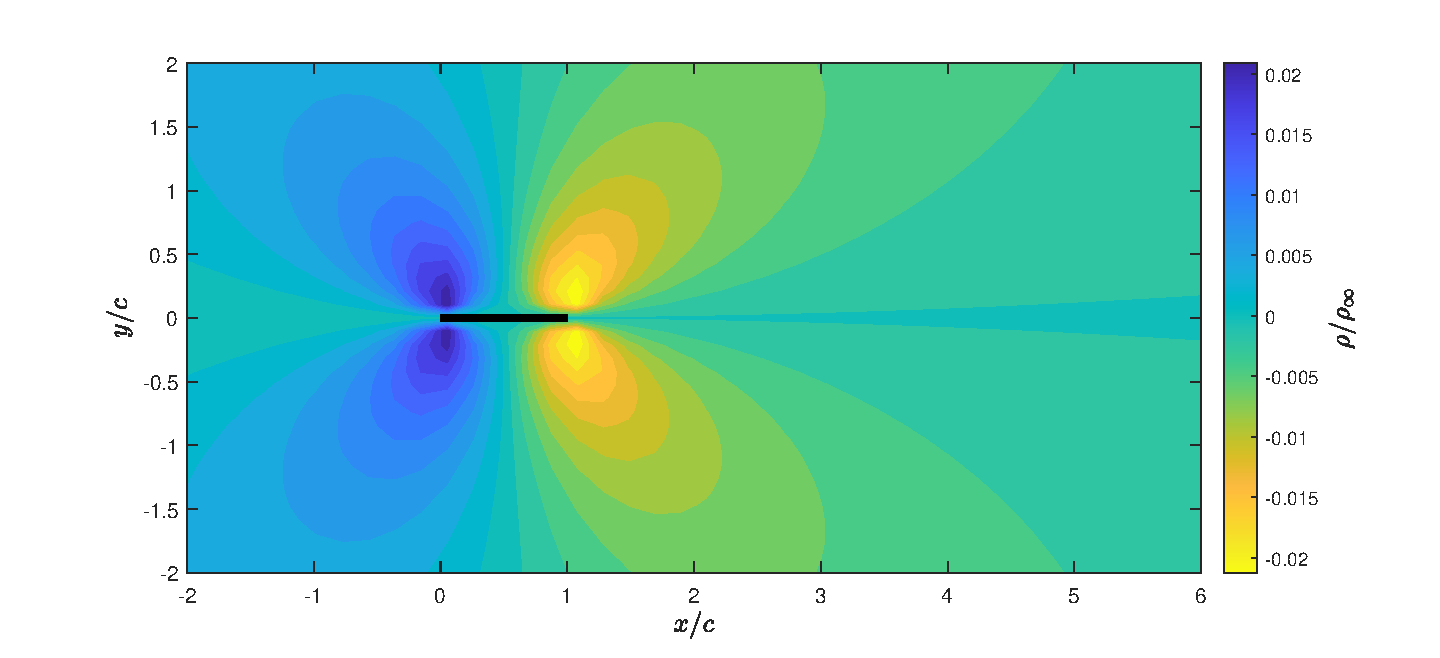
\includegraphics[width=0.58\textwidth]{drawings/SS_U.1_density.eps}
    \vspace{0.07cm}
    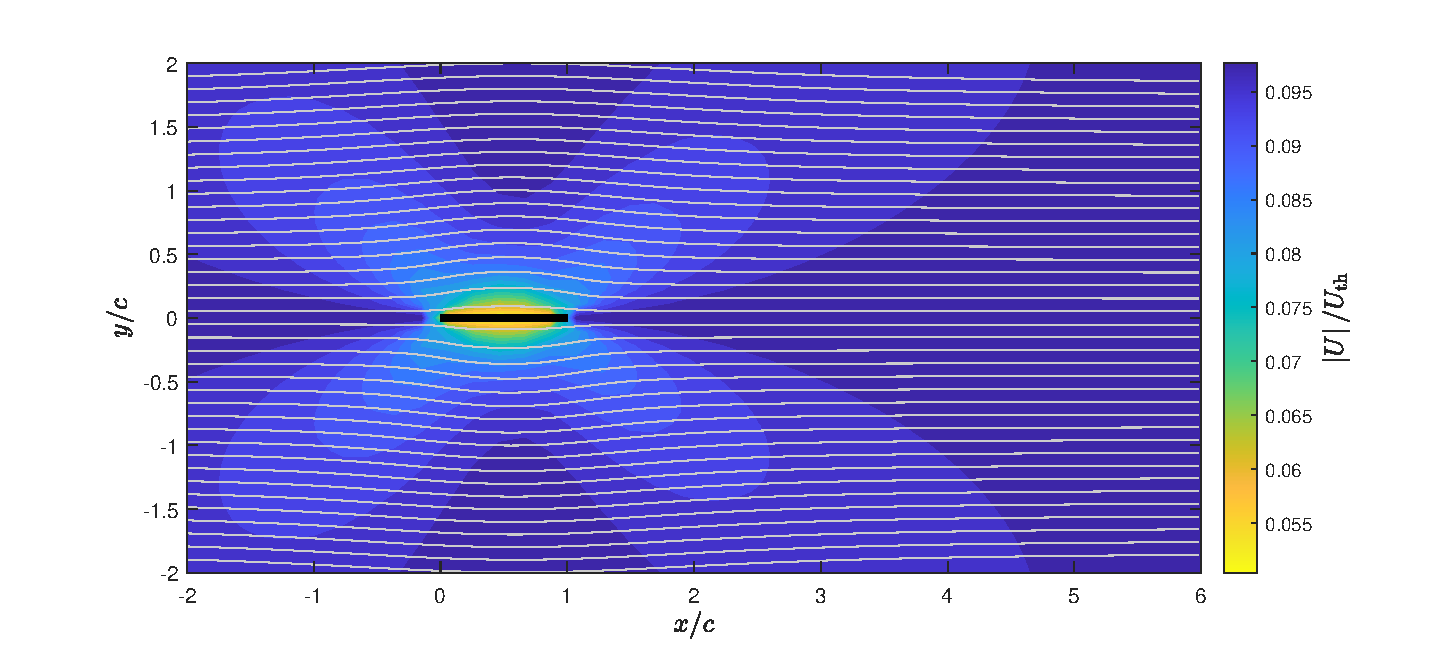
\includegraphics[width=0.58\textwidth]{drawings/SS_U.1_velocity.eps}
    \vspace{0.07cm}
    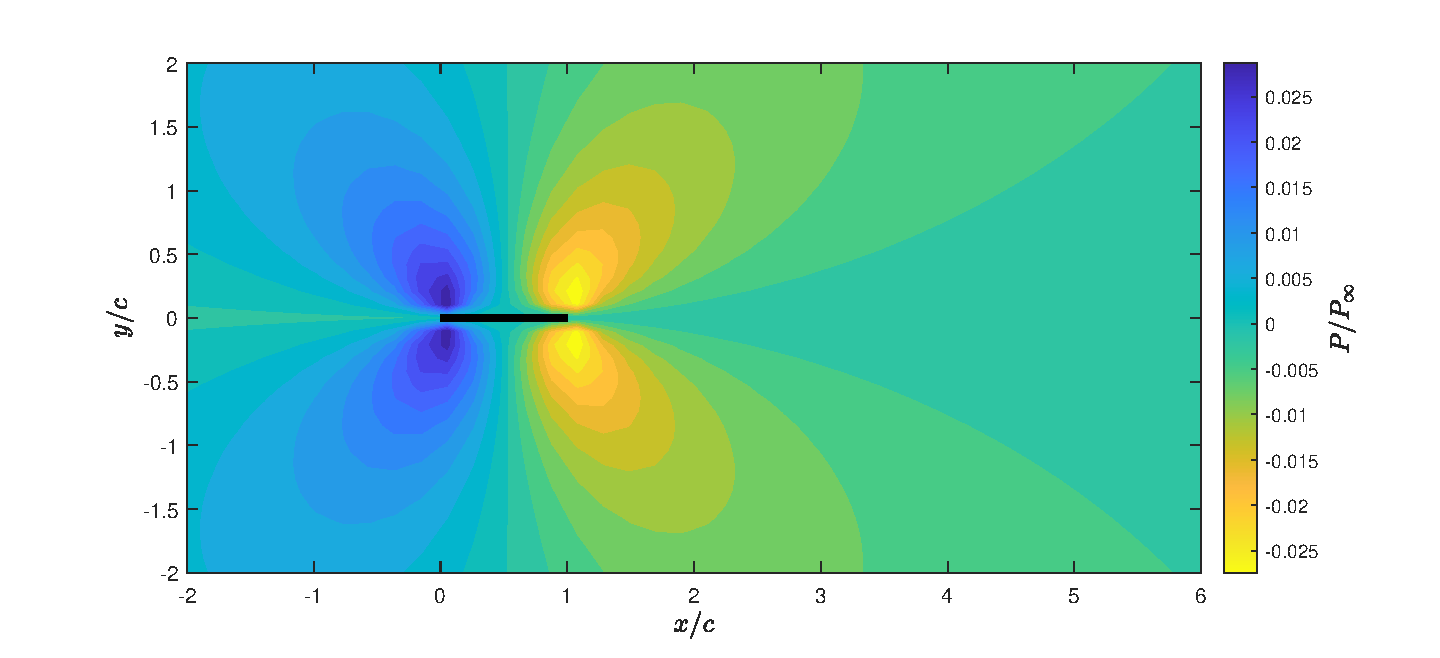
\includegraphics[width=0.58\textwidth]{drawings/SS_U.1_pressure.eps}
    \vspace{0.07cm}
    \begin{minipage}{0.58\textwidth}
    \fbox{%
        \parbox{\dimexpr\linewidth-2\fboxsep-2\fboxrule\relax}{%
            \footnotesize
            Variations of density, velocity and static pressure by \textbf{steady-state} fluid flow of $U_\infty = 0.1$, angle of attack $\alpha=0^{\circ}$
        }%
    }
    \end{minipage}
    \label{fig:steady_state}
\end{wrapfigure}

In this section, we transition from analytical derivations to a more visual representation, showcasing plots derived from the expressions discussed in the preceding section. Our emphasis will be on plots representing steady-state conditions and a specific simple unsteady scenario where the speed is 'Transonic' ($\frac{U_\infty^*}{U_{\mathrm{th}}^*} = \sqrt{U_x^2 + U_y^2} = 1$). In this scenario, the airfoil's temperature exhibits minor oscillations around the distant fluid temperature, and the airfoil's velocity shows slight oscillations around the $x$-axis. While the analytical expressions we've derived offer the flexibility to probe nearly every conceivable state, in this section, we've chosen to spotlight only select, straightforward cases to provide clarity and foundational understanding.

\subsection{Steady-State} \label{sec:Steady-State}
In the steady-state case, we delve into a scenario where the fluid flow velocity is distinctly "subsonic", with a magnitude given by $U_\infty = 0.1$. Here, the airfoil remains stationary along the $x$-axis, and its temperature is set to match the temperature of the distant fluid, ensuring a consistent thermal environment. Notably, the direction of the fluid flow aligns parallel to the orientation of the airfoil, specifically pointing towards the positive $x$-axis direction.

The visual representations in this subsection (Fig. \ref{fig:steady_state}) primarily focus on the variations in the density field, velocity field and static pressure field. These plots capture the difference between the computed density and the normalized density of the fluid flow, as well as the static pressure. As one would anticipate, as we move farther from the airfoil, this difference gradually diminishes, approaching zero. This behavior underscores the consistency and reliability of our analytical models. Additionally, the subsection presents plots showcasing the fluid velocity in close proximity to the airfoil. Another significant inclusion is the depiction of the static pressure difference, contrasting the calculated static pressure against the static pressure of the resting fluid. Together, these visual insights offer a comprehensive understanding of the hydrodynamic fields in the specified steady-state scenario.

\subsection{Unsteady-state}
\begin{wrapfigure}{l}{0.6\textwidth}
\caption{}
    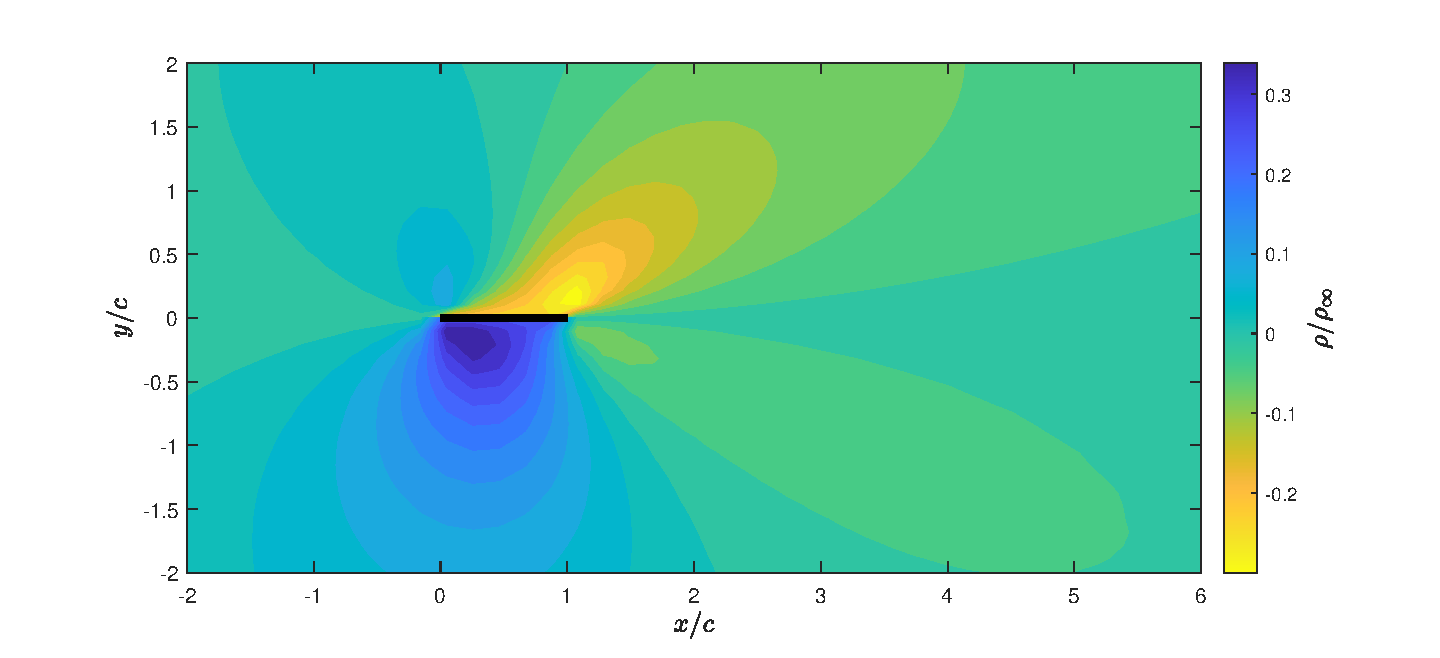
\includegraphics[width=0.58\textwidth]{drawings/U1_alpha10_density.eps}
    \vspace{0.07cm}
    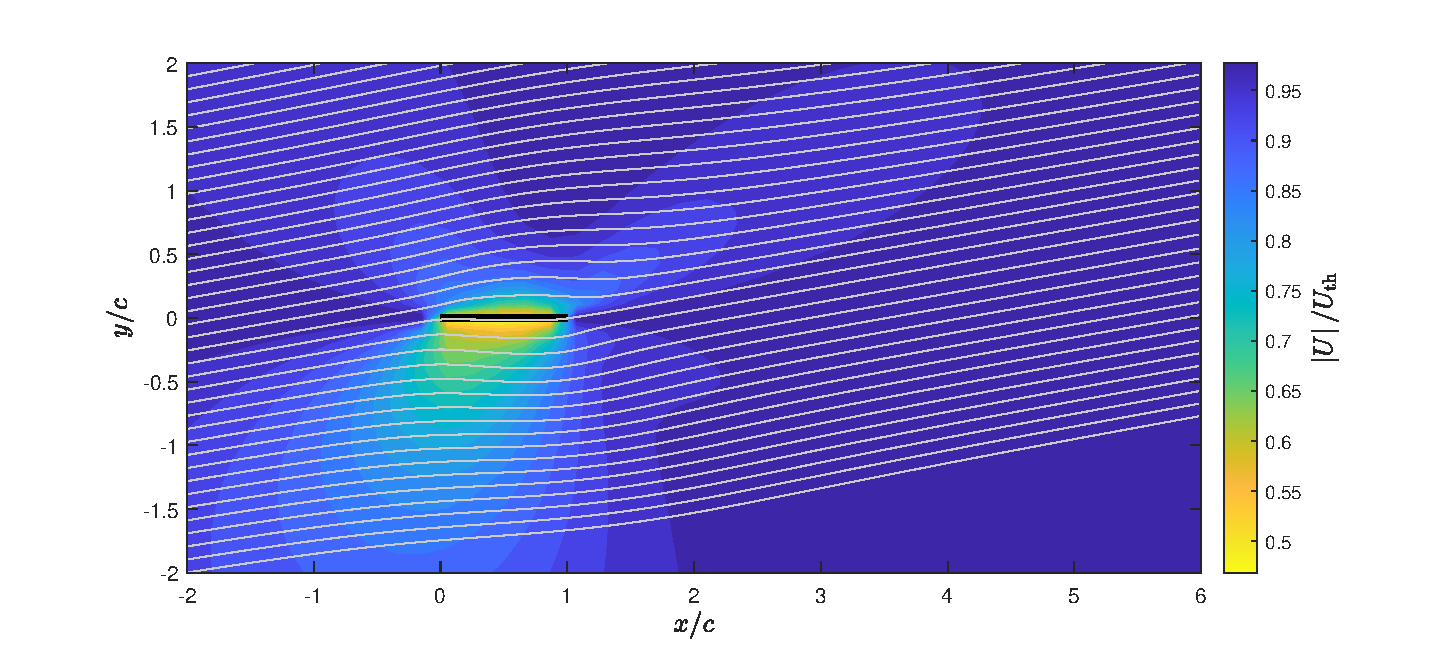
\includegraphics[width=0.58\textwidth]{drawings/U1_alpha10_velocity.eps}
    \vspace{0.07cm}
    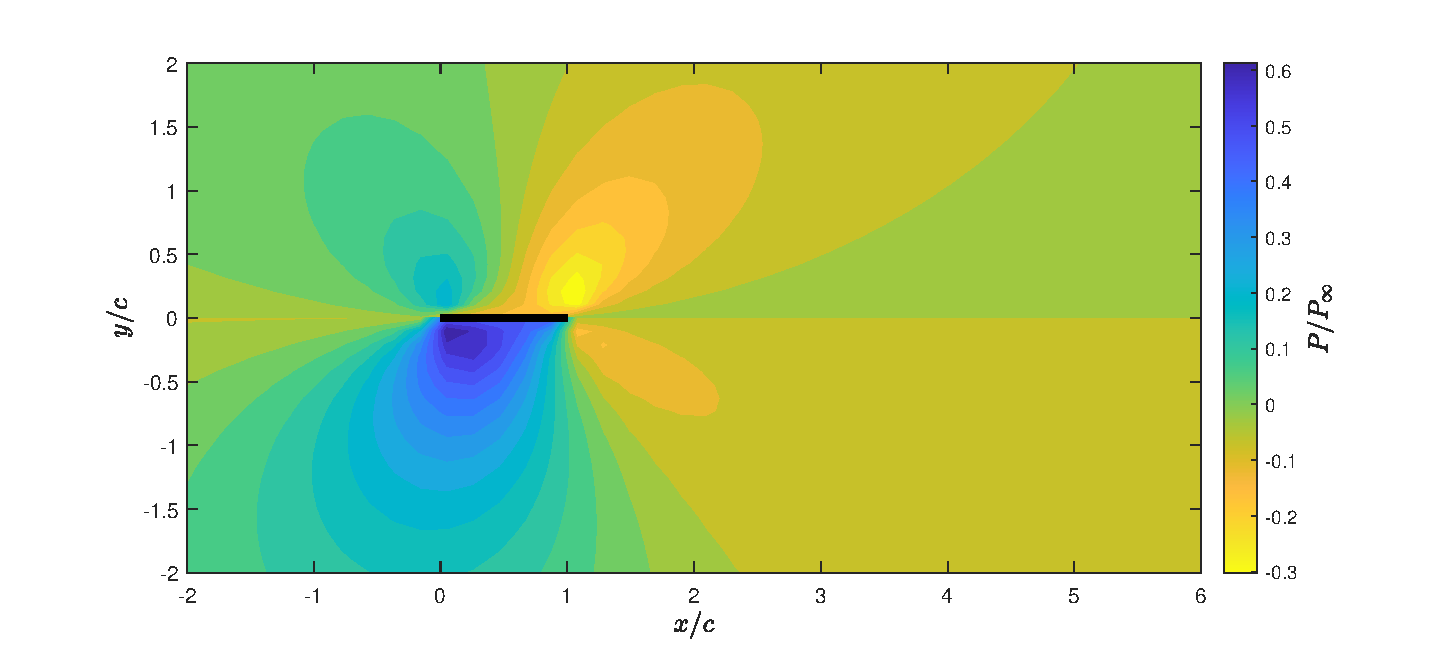
\includegraphics[width=0.58\textwidth]{drawings/U1_alpha10_pressure.eps}
    \vspace{0.07cm}
    \begin{minipage}{0.58\textwidth}
    \fbox{%
        \parbox{\dimexpr\linewidth-2\fboxsep-2\fboxrule\relax}{%
            \footnotesize
            Variations of density, velocity and static pressure by fluid flow of $U_\infty = 1$, angle of attack $\alpha=10^{\circ}$, $T_\af = 1+0.05\sin(t)$, $V_\af = 0.05\sin(t)$
        }%
    }
    \end{minipage}
    \label{fig:unsteady_state}
\end{wrapfigure}
In the unsteady-state case, we venture into dynamic scenarios characterized by "Transonic" speeds, where $U_\infty = 1$. The airfoil, set at an angle of attack of $10$ degrees, exhibits minor oscillations around the distant fluid temperature. Additionally, the airfoil's velocity demonstrates slight oscillations around the $x$-axis, introducing an element of variability. This subsection offers visual representations (Fig. \ref{fig:unsteady_state}) that capture the intricate dynamics of these oscillations, both in terms of temperature and velocity. As we navigate through these plots, readers will gain a deeper understanding of the hydrodynamic fields under transonic and unsteady conditions, emphasizing the nuanced interplay between the airfoil's oscillatory behavior and the surrounding fluid dynamics.

\subsection{Dipole-Induced Dynamics}
\begin{wrapfigure}{r}{0.6\textwidth}
\caption{}
    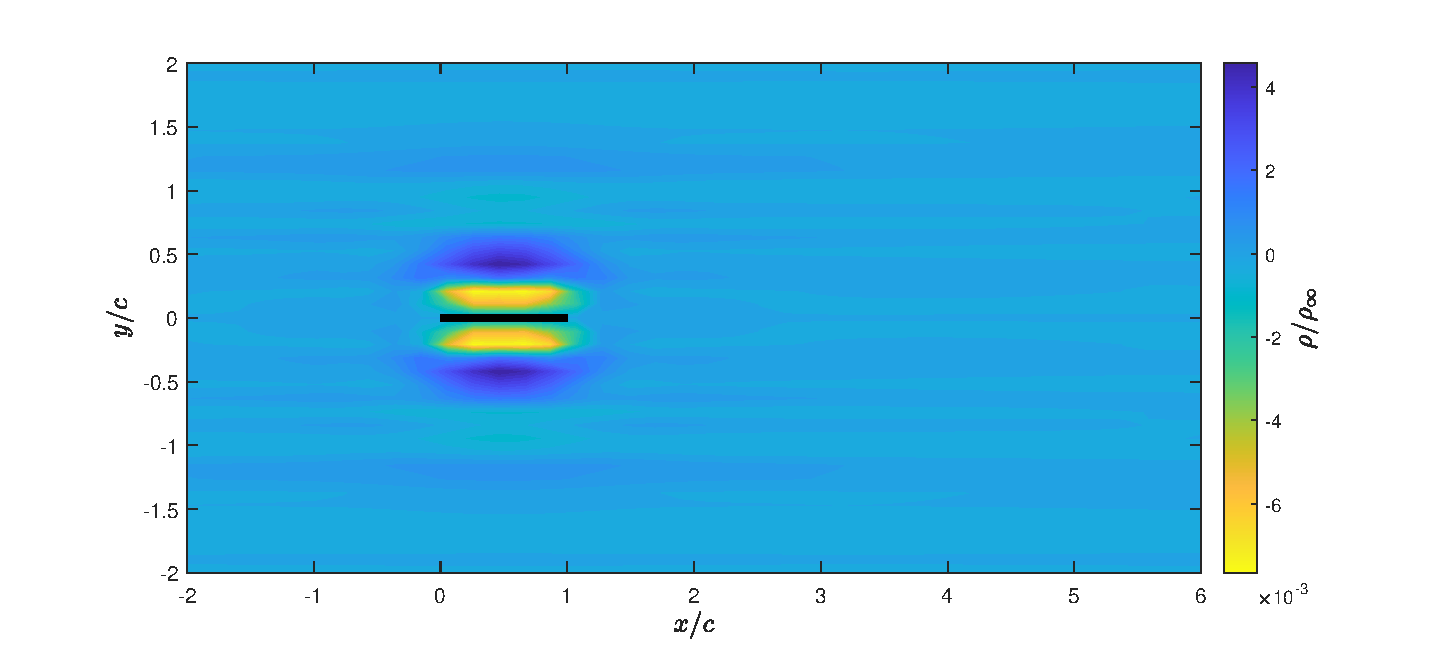
\includegraphics[width=0.58\textwidth]{drawings/U0_epsT.1_omegaT15_density.eps}
    \vspace{0.07cm}
    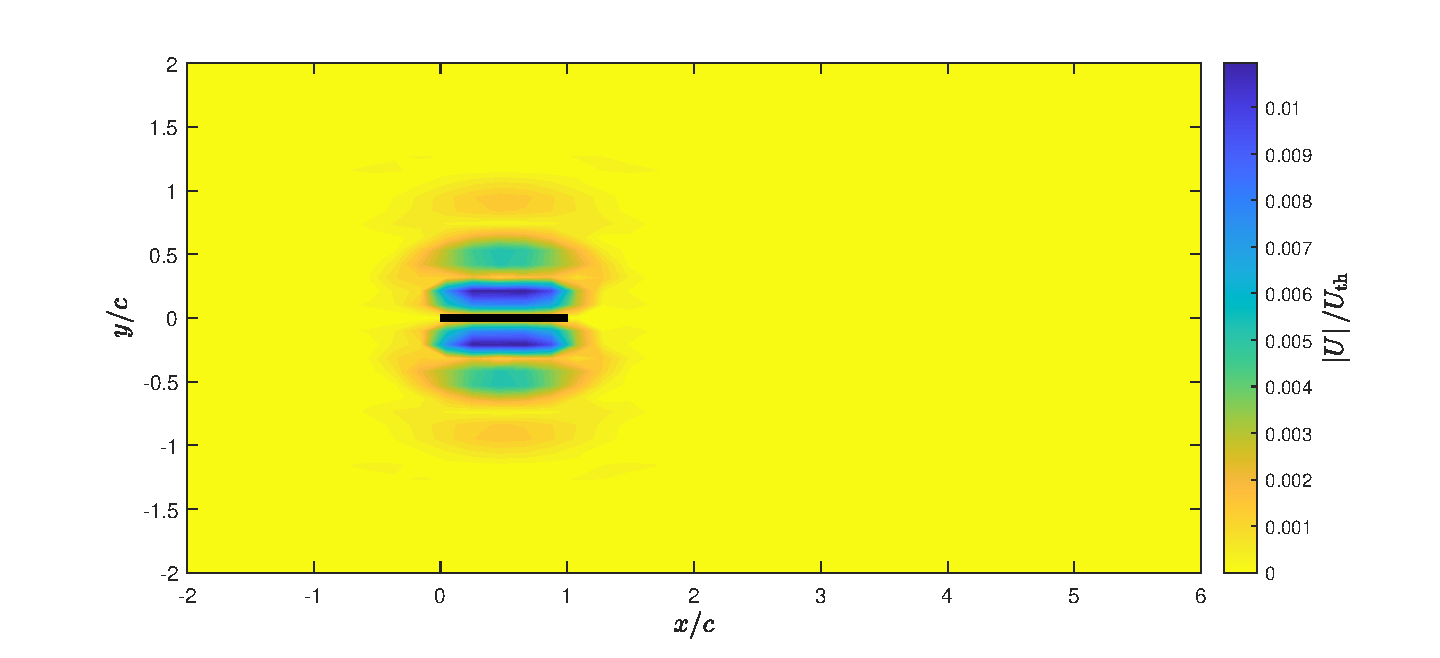
\includegraphics[width=0.58\textwidth]{drawings/U0_epsT.1_omegaT15_velocity.eps}
    \vspace{0.07cm}
    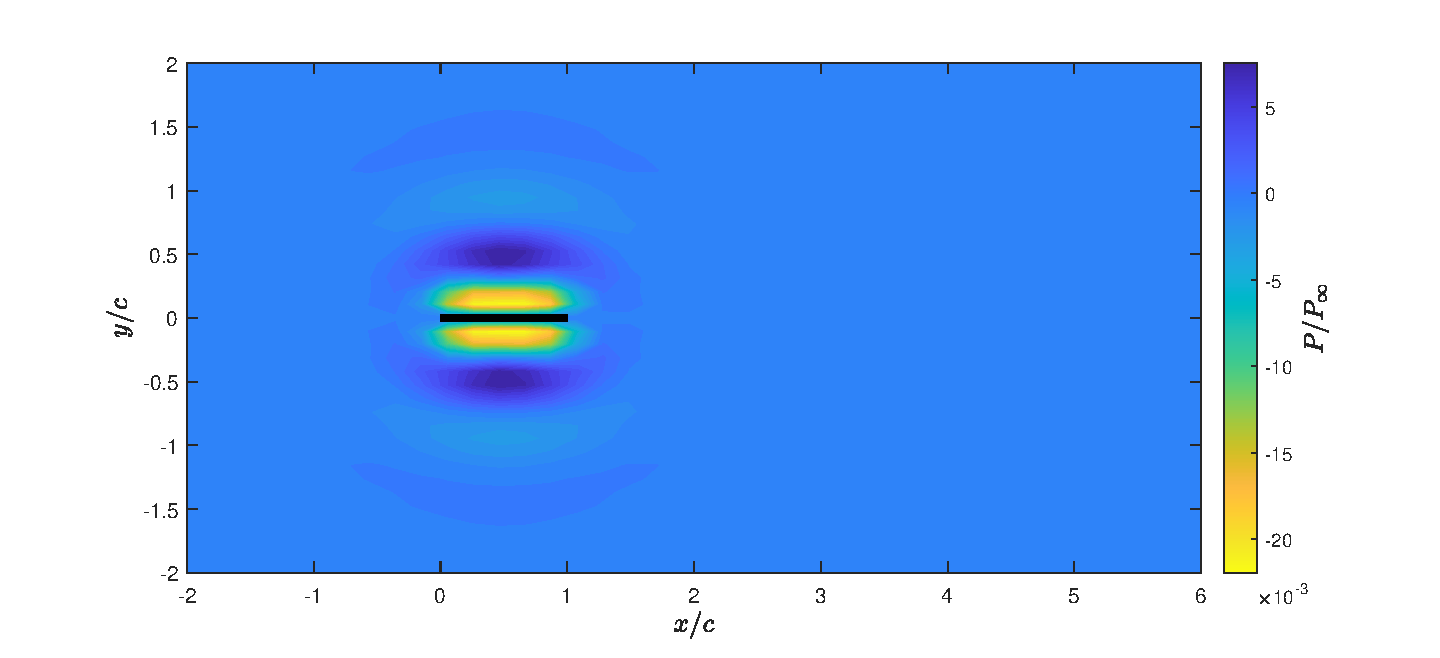
\includegraphics[width=0.58\textwidth]{drawings/U0_epsT.1_omegaT15_pressure.eps}
    \vspace{0.07cm}
    \begin{minipage}{0.58\textwidth}
    \fbox{%
        \parbox{\dimexpr\linewidth-2\fboxsep-2\fboxrule\relax}{%
            \footnotesize
            Variations of density, velocity and static pressure with no fluid flow, but $T_\af = 1+0.1\sin(15t)$ and $V_\af \equiv 0$
        }%
    }
    \end{minipage}
    \label{fig:dipole}
\end{wrapfigure}
In the dipole-induced dynamics case, our exploration shifts towards the hydrodynamic field responses influenced by a dipole source setup. Distinct from both the steady-state and unsteady-state frameworks, this scenario abstains from introducing direct fluid flow. Instead, we perturb the steady conditions by applying alternating heating and cooling regimes to the airfoil. Administered at a notably elevated frequency, these thermal cycles trigger wave formations within the encompassing fluid medium.

The drawings in this section (Fig. \ref{fig:dipole}) mainly show the differences in the density, speed, and pressure of the fluid. These graphical illustrations elucidate the variances between the predicted density and the standardized density of the fluid medium, coupled with the static pressure deviations. Expectedly, the dipole-induced dynamics give rise to wave patterns in the fluid, culminating in palpable shifts within the hydrodynamic landscapes.

By looking into this, we want to better understand how the dipole sources affect the movement of the fluid. This highlights the relationship between the airfoil's heat-related movements and the fluid's behavior.

\section{Lift and Drag}
We shall extend our exploration from the stress tensor results discussed earlier, particularly those in close proximity to the airfoil. Our primary objective here is to derive the lift and drag forces exerted on the airfoil. This analysis is pivotal to the overarching goals of this paper, as it offers a quantitative measure of the aerodynamic performance in the context of unsteady rarefied gas flow. By delving into the intricacies of lift and drag mechanisms, we aim to pave the way for the development of precise prediction models. A key factor influencing these forces, which we will address in detail, is the angle of attack. This comprehensive examination will not only enhance our understanding of the aerodynamic behavior but also solidify the foundational knowledge required for optimizing designs in similar fluidic environments.

For choice of uniform $\displaystyle T_{\text{af}} ,\ V_{\text{af}}$ along $\displaystyle x$:
\begin{equation*}
\begin{aligned}
\text{Noraml Force} =N & =\int\limits _{0}^{1} p_{yy}\left( t,x,0^{-}\right) dx-\int\limits _{0}^{1} p_{yy}\left( t,x,0^{+}\right) dx\\
 & =p_{yy}\left( t,0^{-}\right) -p_{yy}\left( t,0^{+}\right)
\end{aligned}
\end{equation*}
and specifically for $\displaystyle T_{\text{af}} =1$ and $\displaystyle V_{\text{af}} =0$ (that is, pure steady state):
\begin{equation}\label{eq:noraml_force}
N
=
\frac{1}{2}\left[
\left( 2U_{y}^{2}+1 \right) \mathrm{erf} \ U_{y} + 
\frac{2}{\sqrt{\pi }} U_{y} e^{-U_{y}^{2}} +U_{y}\sqrt{\pi }
\right]
.
\end{equation}
Similarly
\begin{equation}\label{eq:tangential_force}
    \begin{aligned}
        \text{Tangential Force} =T & =p_{xy}\left( t,0^{-}\right) -p_{xy}\left( t,0^{+}\right)\\
 & =U_{x}\left( U_{y} \cdotp \mathrm{erf} \ U_{y} +\frac{1}{\mathrm{\sqrt{\pi }}} e^{- U_{y}^{2}}\right)
 .
    \end{aligned}
\end{equation}
Using $\displaystyle N,T$ and the definition of lift (the force acting on a body, perpendicular to the direction of the uniform flow), the lift $\displaystyle L$ would be
\begin{equation}\label{eq:lift}
\begin{aligned}
L & =N\cos \alpha -T\sin \alpha \\
 & =N\frac{U_{x}}{\sqrt{U_{x}^{2} +U_{y}^{2}}} -T\frac{U_{y}}{\sqrt{U_{x}^{2} +U_{y}^{2}}}\\
 & =\frac{U_{x}}{2\sqrt{U_{x}^{2} +U_{y}^{2}}}\left(\mathrm{erf\ } U_{y} +U_{y}\sqrt{\pi }\right)
\end{aligned}
\end{equation}
Finding the maxima of $L$ by calculating the derivative with respect to the angle of attack

\begin{equation}
\frac{dL}{d\alpha } =-\frac{1}{2\sqrt{U_{x}^{2} +U_{y}^{2}}}\left( U_{y}\mathrm{erf\ } U_{y} +U_{y}^{2}\sqrt{\pi } -\frac{2}{\sqrt{\pi }} U_{x}^{2} e^{- U_{y}^{2}} -U_{x}^{2}\sqrt{\pi }\right)
,
\end{equation}
and assuming $\sqrt{U_x^2+U_y^2}\ll1$ 

\begin{equation}
L\approx \frac{1}{2\sqrt{U_{x}^{2} +U_{y}^{2}}}\frac{2+\pi }{\sqrt{\pi }} U_{x} U_{y}
,
\end{equation}
which finally yields
\begin{equation*}
\begin{aligned}
\frac{dL}{d\alpha } & \approx \frac{1}{2\sqrt{U_{x}^{2} +U_{y}^{2}}} \cdot \frac{2+\pi }{\pi }\sqrt{\pi }\left( U_{x}^{2}\mathrm{-} U_{y}^{2}\right)\\
 & =\frac{2+\pi }{2\pi }\sqrt{\pi }\sqrt{U_{x}^{2} +U_{y}^{2}}\cos 2\alpha
\end{aligned}
.
\end{equation*}
Therefore, under theses conditions, the maximum of $L$ is on $\alpha = \frac{\pi}{4}$.

Using Eqs. \ref{eq:noraml_force}, \ref{eq:tangential_force} again, with the definition of drag (the force acting on a body, parallel to the direction of the uniform flow), the drag $D$ shall be

\begin{equation}\label{eq:drag}
D=\frac{1}{\sqrt{U_{x}^{2} +U_{y}^{2}}}\left[\left( U_{y}^{2} +U_{x}^{2}\mathrm{+}\frac{\mathrm{1}}{2}\right) U_{y} \cdotp \mathrm{erf} \ U_{y} +\left( U_{y}^{2} +U_{x}^{2}\right)\frac{1}{\mathrm{\sqrt{\pi }}} e^{-v^{2}} +U_{y}^{2}\sqrt{\pi }\right]
.
\end{equation}
Performing similar analysis under the same assumptions we find that for $\alpha=0$ the drag is linear with the speed of the fluid flow
\begin{equation}
    D \left( \sqrt{U_x^2 + U_y^2} \ll 1 , \alpha=0 \right)
    =
    \sqrt{\frac{U_x^2 + U_y^2}{\pi}}
.
\end{equation}

\begin{figure}[h]
    \centering
    \caption{
    \footnotesize
    Aerodynamic properties as a function of the angle of attack at \( U_\infty = 0.1 \). The upper subplot shows both lift and drag curves, while the lower subplot illustrates the lift over drag ratio, highlighting the optimal angle of attack. The optimal angle of attack, where the lift-to-drag ratio is maximized, is of paramount importance as it indicates the angle at which the airfoil achieves its best aerodynamic efficiency. This optimal efficiency is crucial for the design and performance of aircraft and other aerodynamic structures, especially in the context of unsteady rarefied gas flow, which is the primary focus of this paper.}
    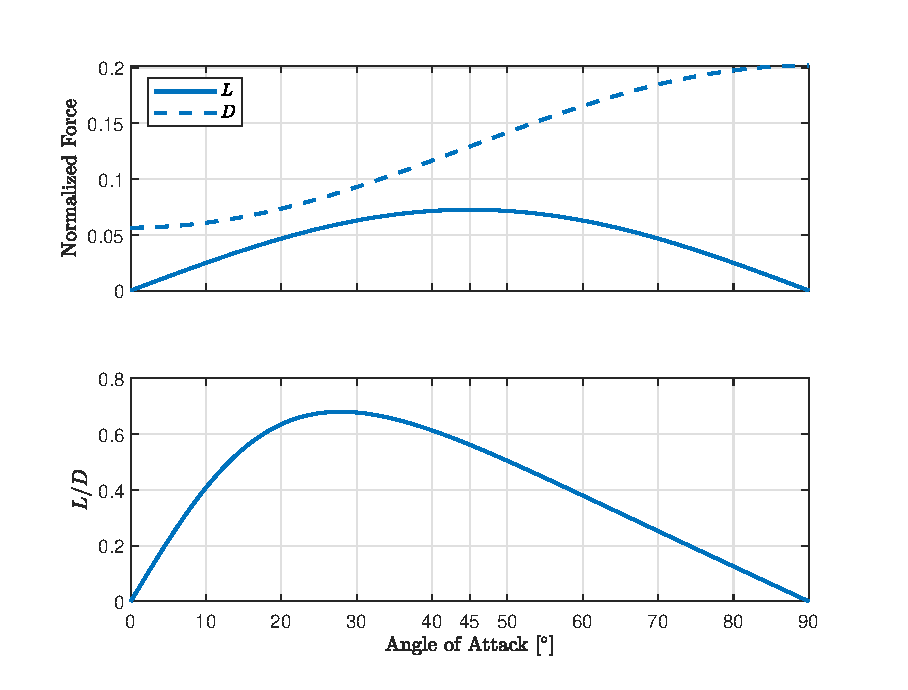
\includegraphics[width=0.8\textwidth]{drawings/U.1_lift_drag.eps}
    \label{fig:aerodynamic_properties_vs_alpha}
\end{figure}

\newpage

\section{Far Field Analysis}
\subsection{Density Wedge}
Examining the density field in a steady flow as depicted in Fig. \ref{fig:steady_state}, we observe a pronounced "wedge" formation subsequent to the trailing edge. Our objective is to probe this manifestation through the derivation of an analytical expression that encapsulates the phenomenon. We shall revisit the general density modulation attributed to the presence of the airfoil (Eq. \ref{eq:density_hitted}):

\begin{equation*}
\rho ^{\text{hitted}}\left(
t,x,y\begin{array}{ c }
\textcolor[rgb]{0,0,1}{\geqslant }\\
\textcolor[rgb]{1,0,0}{\leqslant }
\end{array} 0
\right)
=
\frac{1}{2\sqrt{\pi }}\int\limits _{\textcolor[rgb]{0,0,1}{0} ,\textcolor[rgb]{1,0,0}{-\infty }}^{\textcolor[rgb]{0,0,1}{+\infty } ,\textcolor[rgb]{1,0,0}{0}}\frac{\rho _{\text{af}}\left(\tilde{t}\right)}{\sqrt{T_{\text{af}}\left(\tilde{t}\right)}} e^{-\frac{\left( \xi _{y} -V_{\text{af}}\left(\tilde{t}\right)\right)^{2}}{T_{\text{af}}\left(\tilde{t}\right)}}\left[\mathrm{erf}\left(\frac{\frac{x}{y} \xi _{y}}{\sqrt{T_{\text{af}}\left(\tilde{t}\right)}}\right) -\mathrm{erf}\left(\frac{\frac{x-1}{y} \xi _{y}}{\sqrt{T_{\text{af}}\left(\tilde{t}\right)}}\right)\right] d\xi _{y}
\end{equation*}
When we're dealing with symmetric flow (with zero angle of attack) in a steady state, the complexity of the problem is considerably reduced to
\begin{equation*}
\rho ^{\text{hitted}}\left(
x,y\begin{array}{ c }
\textcolor[rgb]{0,0,1}{\geqslant }\\
\textcolor[rgb]{1,0,0}{\leqslant }
\end{array} 0
\right)
=
\frac{1}{2\sqrt{\pi }}\int\limits _{\textcolor[rgb]{0,0,1}{0} ,\textcolor[rgb]{1,0,0}{-\infty }}^{\textcolor[rgb]{0,0,1}{+\infty } ,\textcolor[rgb]{1,0,0}{0}}e^{-\xi _{y}^{2}}\left[\mathrm{erf} \ \left(\frac{x}{y} \xi _{y}\right) -\mathrm{erf} \ \left(\frac{x-1}{y} \xi _{y}\right)\right] d\xi _{y}
,
\end{equation*}
We then introduce a new variable, denoted by $m=\frac{x}{y}$. By using advanced techniques like the Taylor expansion, we're able to approximate the error function $\mathrm{erf} \ ( z+\delta z)$ around $z$, especially when considering the condition where the vertical distance is significantly large $y \gg 1$. By 1st order approximation
\begin{equation*}
\begin{aligned}
\rho ^{\text{hitted}}\left(
x,y\begin{array}{ c }
\textcolor[rgb]{0,0,1}{\geqslant }\\
\textcolor[rgb]{1,0,0}{\leqslant }
\end{array} 0
\right)
& =
\frac{1}{2\sqrt{\pi }}\int\limits _{\textcolor[rgb]{0,0,1}{0} ,\textcolor[rgb]{1,0,0}{-\infty }}^{\textcolor[rgb]{0,0,1}{+\infty } ,\textcolor[rgb]{1,0,0}{0}}
e^{-\xi _{y}^{2}}\left[\mathrm{erf} \ ( m\xi _{y}) -\mathrm{erf} \ \left( m\xi _{y} -\frac{1}{y} \xi _{y}\right)\right] d\xi _{y}\\
 & \approx \cpm \frac{1}{2\pi y\left( 1+m^{2}\right)}
\end{aligned}
.
\end{equation*}

Finally, by replicating the same method for the particles unaffected by the airfoil, we obtain a full model:
\begin{gather}
\begin{aligned}
\rho\left(
x,y\begin{array}{ c }
\textcolor[rgb]{0,0,1}{\geqslant }\\
\textcolor[rgb]{1,0,0}{\leqslant }
\end{array} 0
\right)\approx
&  \cpm 1 \cmp\frac{1}{2\pi y} e^{-\mu \frac{U_{x}}{m}}\left\{\left( 1+m^{2}\right) e^{-\mu U_{x} m} + \mu \sqrt{\frac{\pi }{1+m^{2}}}\left[ 1+\mathrm{erf} \ \left( \mu \sqrt{1+m^{2}}\right)\right]\right\}\\
 & \cpm\frac{1}{2\pi y\left( 1+m^{2}\right)}
\end{aligned} \\
m=\frac{x}{y} \quad \quad ,\quad \quad \mu =\frac{U_{x} m}{1+m^2}
\nonumber
\end{gather}

In Section \ref{sec:Steady-State}, the steady-state situation was discussed, where the velocity of fluid flow was distinctly in the subsonic range. Additionally, the airfoil was fixed along the x-axis, as visualized in Fig. \ref{fig:steady_state}. Nonetheless, we assumed notably large $y$ values in our current discussion. This implies that the findings from the steady-state scenario might not be of particular interest, as the density "wedge" manifests relatively near the $x$ axis.

As we increase the fluid's velocity, the wedge sharpens and shifts rightwards, indicating an increase in $x$-values. This behavior is illustrated in Fig. \ref{fig:steady_state_superSonic}. The nature of the flow in Fig. \ref{fig:steady_state} might not yield intriguing findings due to its low-speed fluid flow characteristics.
\begin{figure}[H]
    \centering
    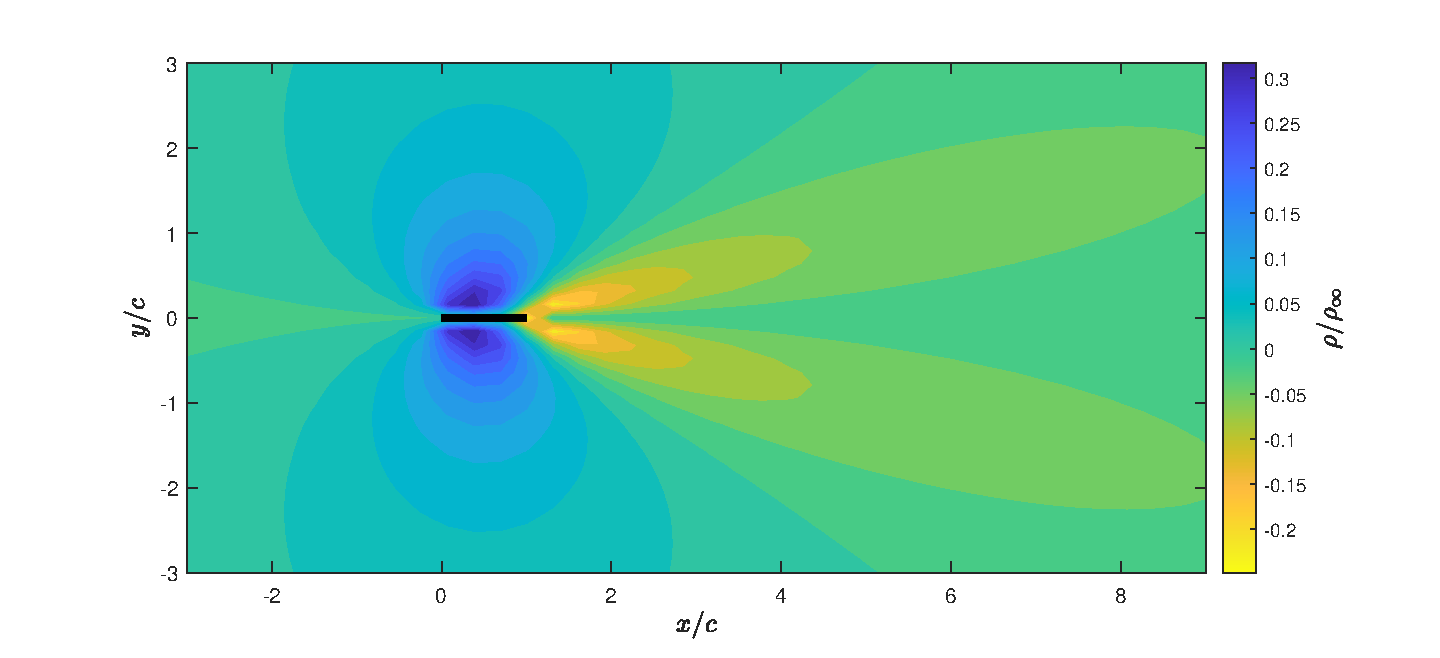
\includegraphics[width=0.7\linewidth]{drawings/SS_U3_density.eps}
    \caption{
        \footnotesize
        Density wedge behavior at steady-state with increased fluid velocity of $U_\infty = 3$, angle of attack $\alpha=0^{\circ}$}
    \label{fig:steady_state_superSonic}
\end{figure}
To further our understanding, we engaged in tests for scenarios where the normalized fluid flow velocity is set at $U_\infty = 3$. This led us to the insights of Fig. \ref{fig:wedge_analysis}, which compare the perturbed density against its mathematical approximation from our earlier discussions and showcases the relative error in percentages. Upon closer inspection of this figure, the error remains under the 1\% mark. Moreover, the way the curves move is very similar, especially where they peak.
\begin{figure}[H]
    \centering
    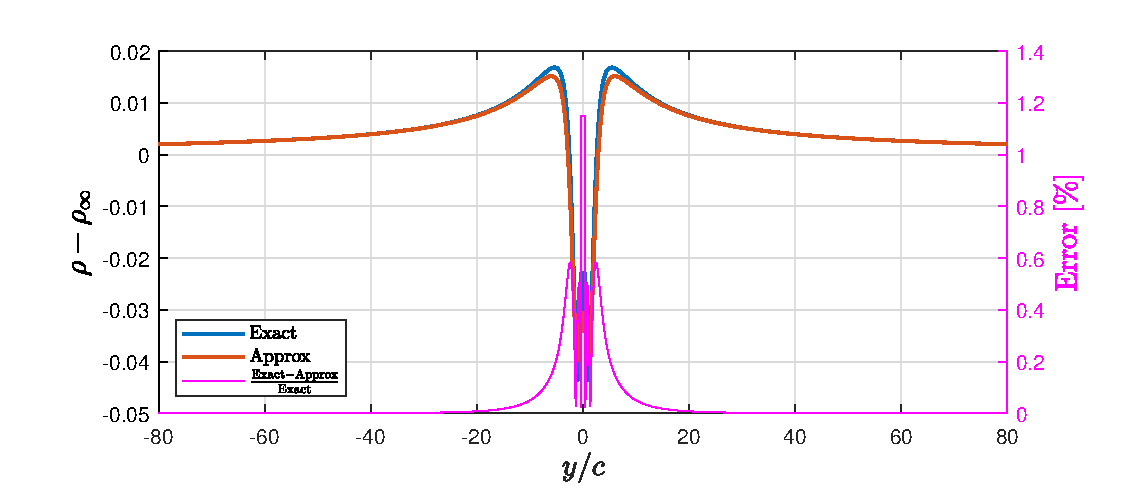
\includegraphics[width=0.7\linewidth]{drawings/WA_U3_x5.eps}
    \caption{\footnotesize Comparison between exact solution and its approximation, including the relative error in percents.}
    \label{fig:wedge_analysis}
\end{figure}

\subsection{Abeam Chord Center}
In this study, attention is directed towards the mid-chord location of the airfoil, denoted at $x=1/2$. Rather than delving into the fluid dynamics surrounding the airfoil, the research primarily explores the thermodynamic reactions evident far above and beneath the airfoil's central region when exclusively subjected to a sinusoidal temperature modulation defined as:
\begin{equation}\label{eq:abeam_chord_center_Taf}
    T_\af (t)
    =
    1+\epsilon \sin (\omega t)
    \qquad
    \epsilon\ll 1
.
\end{equation}

This investigative approach yields profound insights. In scenarios devoid of airfoil movement and fluid interaction, thermal fluctuations can precipitate notable alterations in the fluid's density and stress profiles. By introducing a periodic thermal variation, the study endeavors to outline the responses of thermodynamic fields to temperature shifts. Such methodical adjustments potentially mirror conditions observed in real-world applications. The primary aim of this research is to shed light on the consequences of temperature variations at the airfoil's mid-chord region.

Under the conditions defined in Eq. \ref{eq:abeam_chord_center_Taf} and the following:
\begin{equation*}
\begin{array}{ r r l }
U_x = & U_y & =0\\
 & V_\af (t) & =0
\end{array}
,
\end{equation*}
and recalling Eqs. \ref{eq:density_free} and \ref{eq:density_hitted}, we have
\begin{equation*}
\begin{array}{ r l l }
\rho \left( t,x=1/2,y\begin{array}{ c }
\textcolor[rgb]{0,0,1}{\geqslant }\\
\textcolor[rgb]{1,0,0}{\leqslant }
\end{array} 0\right) & =1 & -\frac{1}{\sqrt{\pi }}\int\limits _{\textcolor[rgb]{0,0,1}{0} ,\textcolor[rgb]{1,0,0}{-\infty }}^{\textcolor[rgb]{0,0,1}{+\infty } ,\textcolor[rgb]{1,0,0}{0}} e^{-\xi _{y}^{2}}\,\erf\left(\frac{1}{2y} \xi _{y}\right) d\xi _{y}\\
 &  & +\frac{1}{\sqrt{\pi }}\int\limits _{\textcolor[rgb]{0,0,1}{0} ,\textcolor[rgb]{1,0,0}{-\infty }}^{\textcolor[rgb]{0,0,1}{+\infty } ,\textcolor[rgb]{1,0,0}{0}}\frac{1}{1+\epsilon \sin\left( \omega \tilde{t}\right)} e^{-\frac{\xi _{y}^{2}}{T_{\text{af}}\left(\tilde{t}\right)}}\mathrm{erf}\left(\frac{\frac{1}{2y} \xi _{y}}{\sqrt{1+\epsilon \sin\left( \omega \tilde{t}\right)}}\right) d\xi _{y}
\end{array}
\end{equation*}
Adopting a first-order Taylor expansion for $\erf z$, $e^{-z^2}$ and $(1+z)^a$, this simplifies further to:
\begin{equation}\label{eq:rho_before_Abramowitz}
\rho \left( t,x=1/2,y\begin{array}{ c }
\textcolor[rgb]{0,0,1}{\geqslant }\\
\textcolor[rgb]{1,0,0}{\leqslant }
\end{array} 0\right) =1\cpm \frac{\epsilon }{\pi y}\int\limits _{0}^{\infty }\left( \xi _{y}^{2} -\frac{3}{2}\right)\sin\left( \omega \tilde{t}\right) \cdot \xi _{y} e^{-\xi _{y}^{2}} d\xi _{y}
.
\end{equation}
To derive a general solution for the following form,
\begin{equation*}
    \begin{aligned}
        I_m & =\int\limits_{0}^{\infty} \left( \xi_y^2 - \frac{3}{2} \right) \sin\left( \omega \tilde{t} \right) \cdot \xi_y^m e^{-\xi_y^2} d\xi_y & \\
        & =\Im \left\{e^{i\omega t}\left[\int\limits _{0}^{\infty } \xi _{y}^{m+2} e^{-\xi _{y}^{2} -z/\xi _{y}} d\xi _{y} -\frac{3}{2}\int\limits _{0}^{\infty } \xi _{y}^{m} e^{-\xi _{y}^{2} -z/\xi _{y}} d\xi _{y}\right]\right\}
\end{aligned}
,
\end{equation*}
we invoke the Abramowitz method \cite{abramowitz1953evaluation}, which gives the asymptotic estimate of the integral as:
\begin{gather*}
J_{n}( z) =\int\limits _{0}^{\infty } s^{n}\exp\left( -s^{2} -z/s\right) ds=3^{-n/2} \zeta ^{n/2}\exp( -\zeta )\sqrt{\frac{\pi }{3}}\left[ 1+\frac{a_{n}^{( 1)}}{\zeta } +\frac{a_{n}^{( 2)}}{\zeta ^{2}} +\cdots \right]\\
z=i\omega y\quad \quad ,\quad \quad | z| \gg 1\quad \quad ,\quad \quad \zeta =3( z/2)^{2/3}\\
a_{n}^{( 1)} =\left( 3n^{2} +3n-1\right) /12\\
a_{n}^{( 2)} =\left( 9n^{4} +6n^{3} -51n^{2} -24n+25\right) /288
\end{gather*}
Thus, the approximate solution can be expressed as:
\begin{equation}\label{eq:I_m}
\begin{aligned}
    I_m & =\int\limits_0^\infty \left( \xi_y^2 - \frac{3}{2} \right) \sin\left( \omega\tilde{t} \right) \cdot \xi_y^m e^{-\xi_y^2} d\xi_y \\
     & =
     \Im \left\{ e^{i\omega t}\left[ J_{m+2}(z) - \frac{3}{2} J_{m}(z) \right]\right\}
\end{aligned}
.
\end{equation}
With the above formulation, it becomes feasible to determine Eq. \ref{eq:rho_before_Abramowitz} using the relation from Eq. \ref{eq:I_m}:

\begin{multline}
\rho \left( t,x=1/2,y\begin{array}{ c }
\textcolor[rgb]{0,0,1}{\geqslant }\\
\textcolor[rgb]{1,0,0}{\leqslant }
\end{array} 0\right)
\approx
1-\frac{1}{2\pi y} \cpm \\
\cpm \left\{\frac{1}{2\pi y} + \epsilon \frac{\omega }{8\Omega \sqrt{3\pi }} e^{-\frac{3}{2} \Omega }\left[( 4\Omega -3)\cos\left( \omega t-\frac{3\sqrt{3}}{2} \Omega \right) -3\sqrt{3}\sin\left( \omega t-\frac{3\sqrt{3}}{2} \Omega \right)\right]\right\}
\end{multline}
Utilizing the extensive application of \( \Omega =\left(\omega y/2\right)^{2/3} \), we proceed to compute values for \( p_{xx} \), \( p_{yy} \), and \( p_{zz} \):
while making extensive use of the notation $\Omega =\left(\omega y/2\right)^{2/3}$. We can now advance to the calculations for $p_{xx}$, $p_{yy}$ and $p_{zz}$:

\begin{multline}
p_{xx}\left( t,x=1/2,y\begin{array}{ c }
\textcolor[rgb]{0,0,1}{\geqslant }\\
\textcolor[rgb]{1,0,0}{\leqslant }
\end{array} 0\right)
\approx
\frac{1}{2} -\frac{1}{16\pi y^{3} +4\pi y} \cpm \\
\cpm \left\{\frac{1}{16\pi y^{3}} +\epsilon \frac{\omega }{y^{2} \cdotp 2^{16/3}}\frac{1}{\sqrt{3\pi }} e^{-\frac{3}{2} \Omega }\left[\frac{2\Omega -3}{2}\cos\left( \omega t-\frac{3\sqrt{3}}{2} \Omega \right) -\sqrt{3} \Omega \sin\left( \omega t-\frac{3\sqrt{3}}{2} \Omega \right)\right]\right\}
\end{multline}

\begin{multline}
p_{yy}\left( t,x=1/2,y\begin{array}{ c }
\textcolor[rgb]{0,0,1}{\geqslant }\\
\textcolor[rgb]{1,0,0}{\leqslant }
\end{array} 0\right)
\approx
\frac{1}{2} -\frac{1}{2\pi y} \cpm \\
\cpm \left\{\frac{1}{2\pi y} +\epsilon \frac{\omega }{8\Omega \sqrt{3\pi }} e^{-\frac{3}{2} \Omega }\left[( 4\Omega -3)\cos\left( \omega t-\frac{3\sqrt{3}}{2} \Omega \right) -3\sqrt{3}\sin\left( \omega t-\frac{3\sqrt{3}}{2} \Omega \right)\right]\right\}
\end{multline}

\begin{multline}
p_{zz}\left( t,x=1/2,y\begin{array}{ c }
\textcolor[rgb]{0,0,1}{\geqslant }\\
\textcolor[rgb]{1,0,0}{\leqslant }
\end{array} 0\right)
\approx
\frac{1}{2} -\frac{1}{4\pi y} \cpm \\
\cpm \left\{\frac{1}{4\pi y} +\epsilon \frac{\omega }{16\Omega \sqrt{3\pi }} e^{-\frac{3}{2} \Omega }\left[( 4\Omega -1)\cos\left( \omega t-\frac{3\sqrt{3}}{2} \Omega \right) -\sqrt{3}\sin\left( \omega t-\frac{3\sqrt{3}}{2} \Omega \right)\right]\right\}
\end{multline}

We are now set to present a comprehensive visualization of our findings. By juxtaposing the results derived from our model against the analytical solutions for both density and pressure, we aim to emphasize the efficacy and precision of our approximation. As we navigate through the comparative graphs and figures, the closeness of our evaluation to the analytical benchmarks should provide compelling evidence of the adequacy of our approximation. The objective is to convincingly demonstrate that, despite being an approximation, our methodology provides insights that align closely with the established analytical solutions.

\begin{figure}[H]
    \centering
    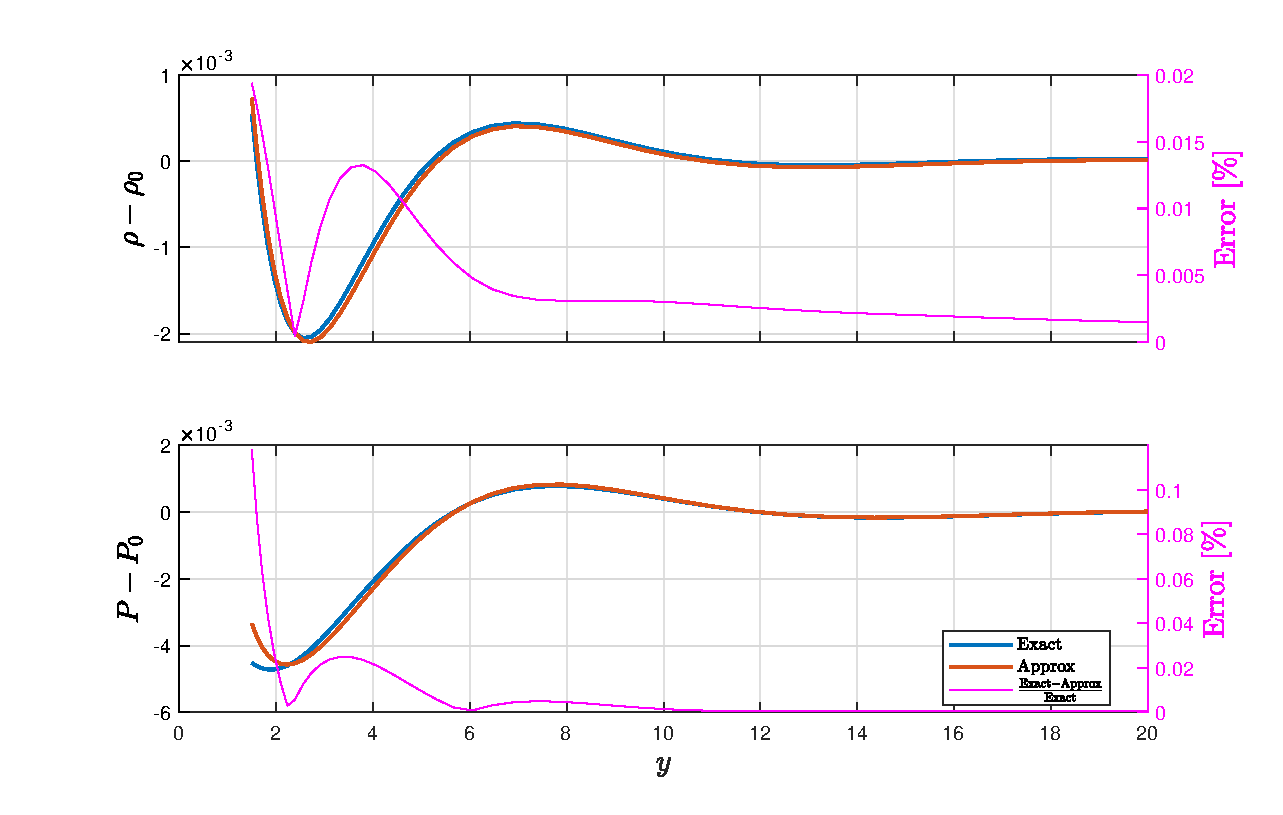
\includegraphics[width=0.8\textwidth]{drawings/ACC.eps} 
    \caption{\footnotesize{Comparison of the exact and approximated solutions. The results for negative $y$ values are not shown due to symmetry with respect to $y=0$. The perturbation follows Eq. \ref{eq:abeam_chord_center_Taf} with $\epsilon = 0.1$ and $\omega = 1$. The upper subplot depicts the density field with the hydrodynamic field on the left $y$-axis and the relative error on the right $y$-axis. The subplot below corresponds to the pressure field, again highlighting the hydrodynamic field on the left $y$-axis and the relative error on the right $y$-axis.}}
    \label{fig:ACC_comparison}
\end{figure}
The visualization on Fig. \ref{fig:ACC_comparison} underscores a commendable alignment between the approximation and the exact solution. Delving deeper into the relative error, it remains significantly beneath the $1\%$ threshold, solidifying the precision of our approximation. A noteworthy observation is the gradual diminishment of the relative error as the values of $y$ escalate. Specifically, beyond $5$ chord lengths, the approximation's relative error becomes nearly indiscernible, closely converging to zero. This reinforces the robustness of our approximation, especially for larger $y$ values.
\chapter{Conclusion}
\section{Conclusion}

The comprehensive examination of hydrodynamic patterns around a flat airfoil in unsteady flow presented in this study enriches our understanding of fluid mechanics. One of the primary endeavors was to elucidate the unsteady rarefied gas dynamics over a flat airfoil using intricate analytical techniques, and this investigation has notably enhanced our insights into the hydrodynamic fields. Given the pivotal nature of such investigations for spacecraft and high-altitude aircraft design, the significance of this research is manifold.

By developing an exact solution for the hydrodynamic fields within the ballistic limit, we have managed to address a broad spectrum of velocities, spanning from subsonic to ultrasonic regimes. This study's findings further underscored the intriguing behavior of hydrodynamic fields around an airfoil, especially when subjected to temperature variations or vertical velocities, culminating in the observation of dipole-induced dynamics (Fig. \ref{fig:dipole}). Additionally, the profound analysis of lift and drag dynamics as a function of angle of attack offers a promising platform for future aerodynamic explorations and optimizations.

From a methodological vantage point, the two-dimensional configuration paired with the normalization of magnitudes facilitated a comprehensive portrayal of the gas state. The dimensionless Boltzmann equation, particularly in the high Knudsen number regime, emerged as an instrumental tool in understanding the behavior of rarefied gases surrounding the airfoil, as indicated by Eqs. \ref{eq:Boltzman}, \ref{eq:macro_number_density}, \ref{eq:macro_velocity} and \ref{eq:macro_stress}. Notably, to determine the airfoil functions $\rho_\af^\pm(t,x)$ as delineated in Eq. \ref{eq:phi}, we imposed an impermeability condition on the normal velocity component $v(t,x,y)$.

Among the paramount findings, our observations during symmetric and steady-state flows highlighted a unique phenomenon, often referred to as the "density wedge." Evident in Fig. \ref{fig:steady_state} and Fig. \ref{fig:steady_state_superSonic}, this wedge characterizes a distinct variation in the density hydrodynamic field, resembling a wedge or a "V" shape behind the trailing edge of the airfoil. Our rigorous efforts enabled us to approximate this behavior with remarkable accuracy, especially for large $y$ values as showcased in Fig. \ref{fig:wedge_analysis}. 
Furthermore, our exploration into the density and static pressure fields on the line $x=1/2$ — abeam the chord center — allowed for the development of accurate approximations of these fields for large $y$ values, as depicted in Fig. \ref{fig:ACC_comparison}. 
Such insights hold profound implications, especially in the context of foreseeing far-field density and static pressure for specific challenges. By potentially neutralizing dynamic effects acting upon the airfoil.

While this research provides a robust foundation, the absence of a comparative analysis with other conditions or geometries signifies an area ripe for future exploration. There exists a pressing need to juxtapose these analytical insights with numerical approaches, such as DSMC, and the potential revelations from continuum limits.

On the practical front, the implications of this research extend far into the domain of aerospace engineering. The ability to theoretically predict lift and drag for flat airfoils in ballistic conditions stands as a testament to the study's relevance. Furthermore, the insights gained into neutralizing dynamic effects present promising prospects for reducing both power consumption and noise, especially in applications such as MEMS sensors.

However, the journey was not devoid of challenges. Navigating through a myriad of parameter permutations presented its set of complexities, suggesting potential avenues that remain unexplored.

In conclusion, this research stands as a monumental stride in the realm of rarefied gas dynamics, presenting both profound insights and opening doors for further explorations in fluid mechanics.


\bibliographystyle{IEEEtran}
\bibliography{refs.bib}


\end{document}